% Chapter 4

\chapter{Resultados} % Chapter title

\label{ch:resultados} % For referencing the chapter elsewhere, use \autoref{ch:mathtest}

%----------------------------------------------------------------------------------------


\section{La importancia del AGN en los modelos de formaci\'on de galaxias}
Uno de los desaf\'ios actuales al cual se enfrentan los modelos de formaci\'on de galaxias, en lo que 
respecta a las galaxias masivas, consiste en controlar el excesivo enfriamento del gas para as\'i evitar tasas 
de formaci\'on estelar por encima de los valores que se observan en el Universo. En la actualidad, se sabe que los 
c\'alculos efectuados sin incluir una inhibici\'on eficiente al ensamblaje de la masa estelar en el rango de masas altas 
de la funci\'on de masa, donde el feedback de supernovas se vuelve ineficiente, lleva a una sobre predicci\'on de la masa 
estelar en estos sistemas por un factor $\sim$10 (ej, Benson et al. 2003).

El {\it feedback} de supernovas, utilizado en los modelos para controlar la formaci\'on estelar en galaxias,
deja de ser eficiente en aquellas m\'as masivas, en particular en las BCGs, en donde una fuente adicional de calentamiento 
para el gas se hace necesaria, siendo la soluci\'on m\'as prometente el {\it feedback} proveniente de la actividad AGN.

Sorprendentemente, este proceso f\'isico ha sido ignorando en los c\'alculos presentes en los modelos de formaci\'on de galaxias durante
mucho tiempo. Sin embargo, desde hace aproximadamente una d\'ecada, su uso en modelos semianal\'iticos 
y en simumlaciones num\'ericas hidrodin\'amicas, ha crecido progresivamente 
(ej. Granato et al. 2004; Springel, Di Matteo $\&$ Hernquist 2005; Bower et al. 2006; Croton et al. 2006; Monaco,
Fontanot $\&$ Taffoni 2007; Sijacki et al. 2007; Somerville et al. 2008; Fabjan et al. 2010; McCarthy et al. 2010;
Martizzi, Teyssier $\&$ Moore 2012; Ragone-Figueroa et al. 2013; Dubois et al. 2014, Martizzi et al. 2016; Bah\'e et al. 2017;
Pillepich et al. 2017).

En el campo de las simulaciones num\'ericas, el uso del {\it feedback} de AGN reduce la masa estelar de las galaxias BCGs
en un factor que var\'ia de 2 a 10 dependiendo del modelo y de la masa de la galaxia considerada (Sijacki et al. 2007; Martizzi 
et al. 2012; Stott et al. 2012; Dubois et al. 2013; Ragone-Figueroa et al. 2013). No obstante, como se ver\'a en \ref{sec:zeta0} el contenido 
estelar de estas galaxias simuladas sigue siendo alto comparado con las masas que miden las observaciones.


En la Fig.
%~\ref{fig:} XXXX 
puede verse el impacto del modelo de {\it feedback} de AGN usado en estas simulaciones sobre las
masas finales (a $z=0$) de dos BCGs y sus respectivos c\'umulos, uno en la muestra de alta masa y otro en la muestra de baja masa. 
En ambos casos la disminuci\'on de la masa final al encender el AGN en la simulaci\'on es evidente.


\begin{figure}[H]
 \hspace*{-0.5cm}
 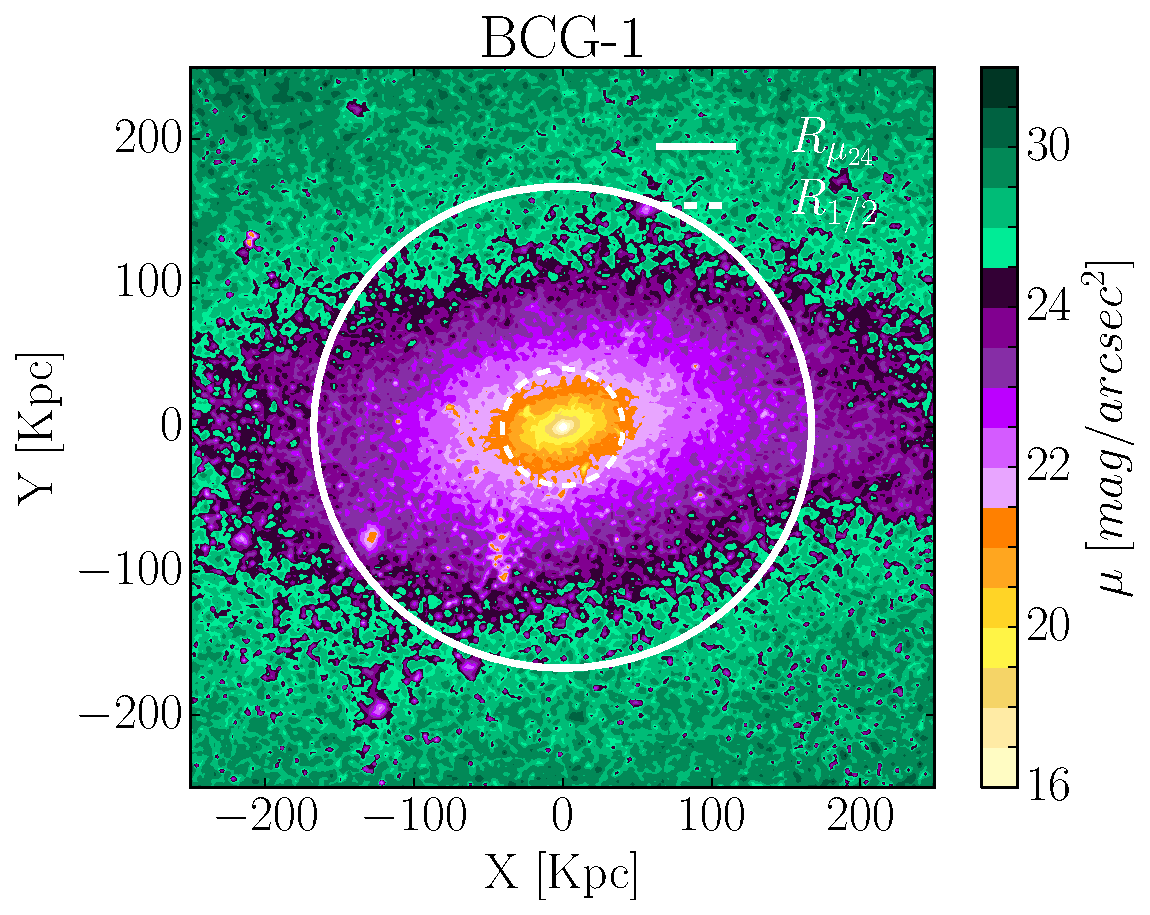
\includegraphics[height=7cm, width=9.0cm, trim={0cm 2.1cm 3.3cm 1cm},clip]{../al_final/LR/LR_CSF/nodust/grupo0/mu24/D1/091/maps_D1_aperturas.pdf}
 \hspace*{-0.27cm}
 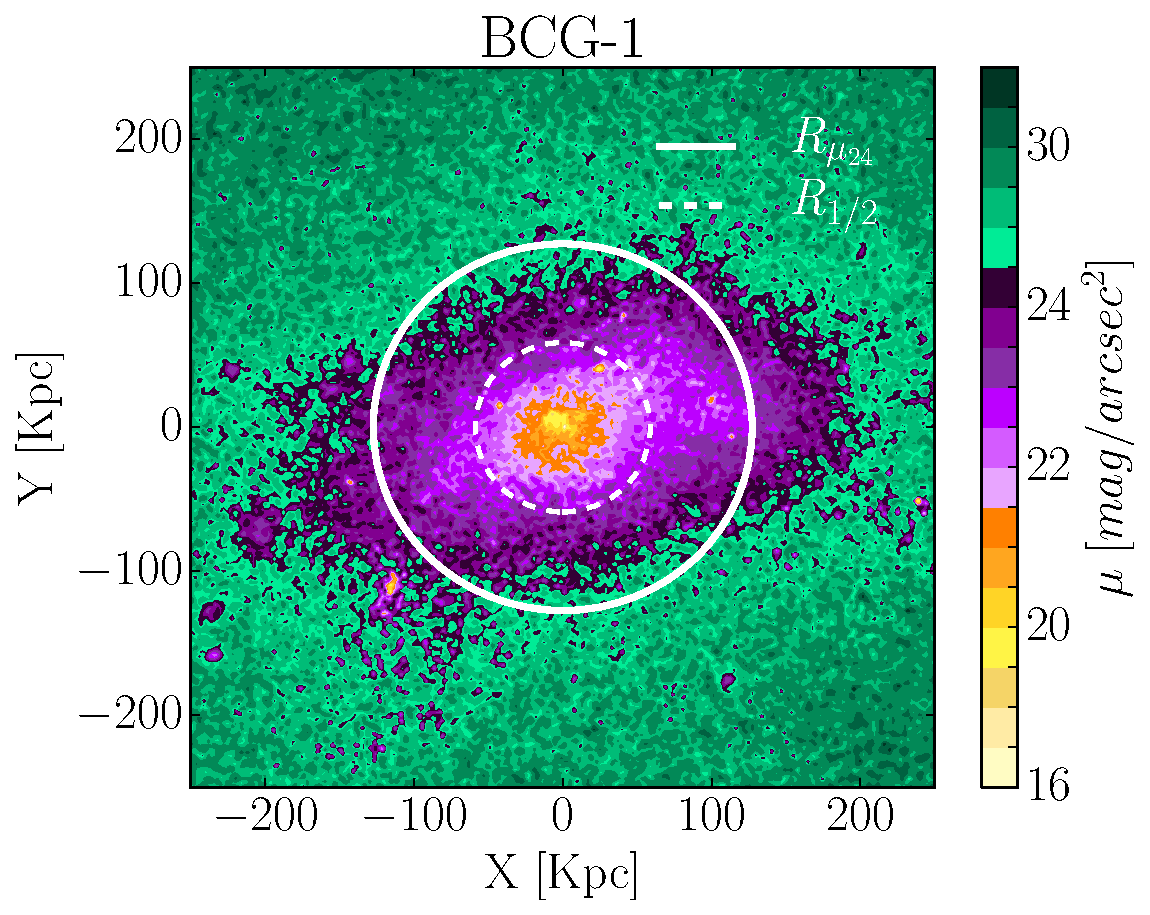
\includegraphics[height=7cm, width=9.0cm, trim={3.2cm 2.1cm 0cm 1cm},clip]{../al_final/LR/LR_minpot3_rmmax/nodust/grupo0/mu24/D1/091/maps_D1_aperturas.pdf}
 \\
  \hspace*{-0.5cm}
 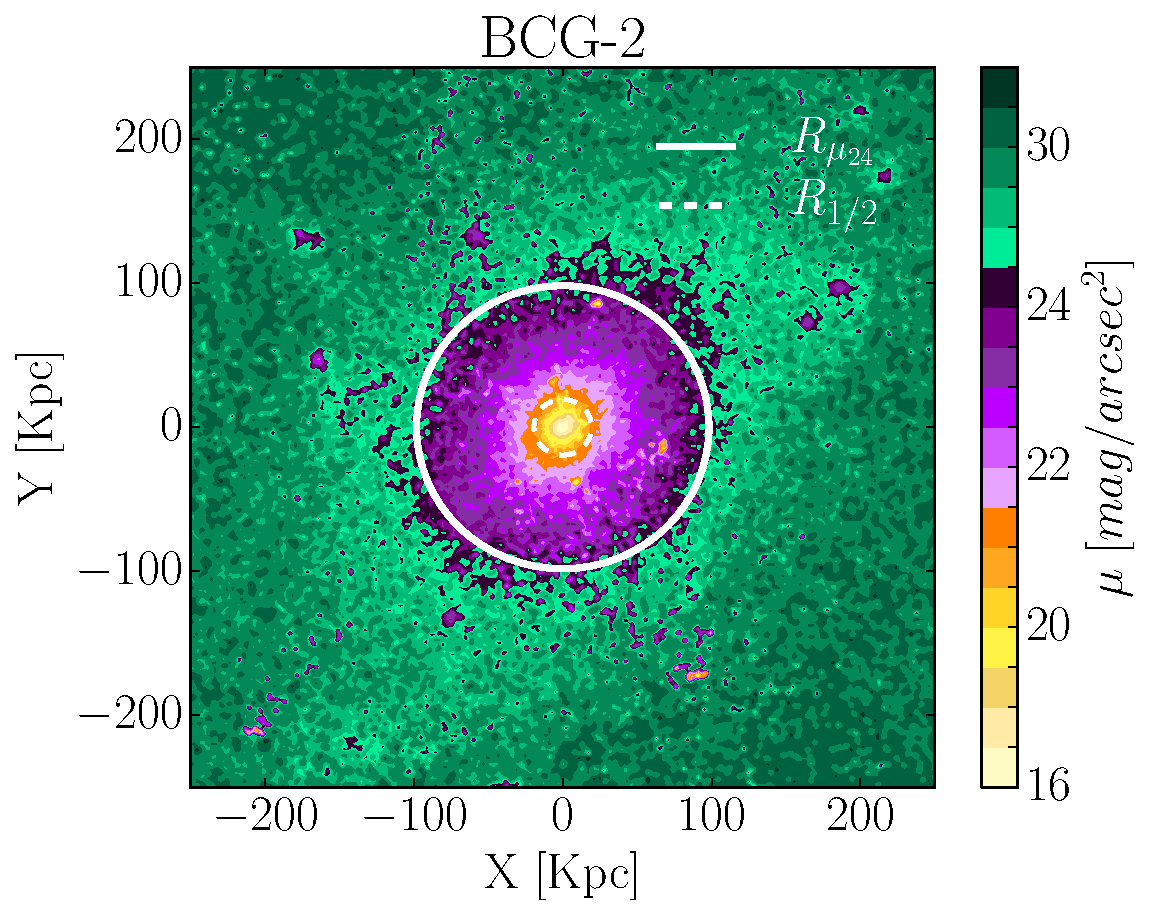
\includegraphics[height=8cm, width=9.0cm, trim={0cm 0cm 3.3cm 1.1cm},clip]{../al_final/LR/LR_CSF/nodust/grupo0/mu24/D2/091/maps_D2_aperturas.pdf}
 \hspace*{-0.27cm}
 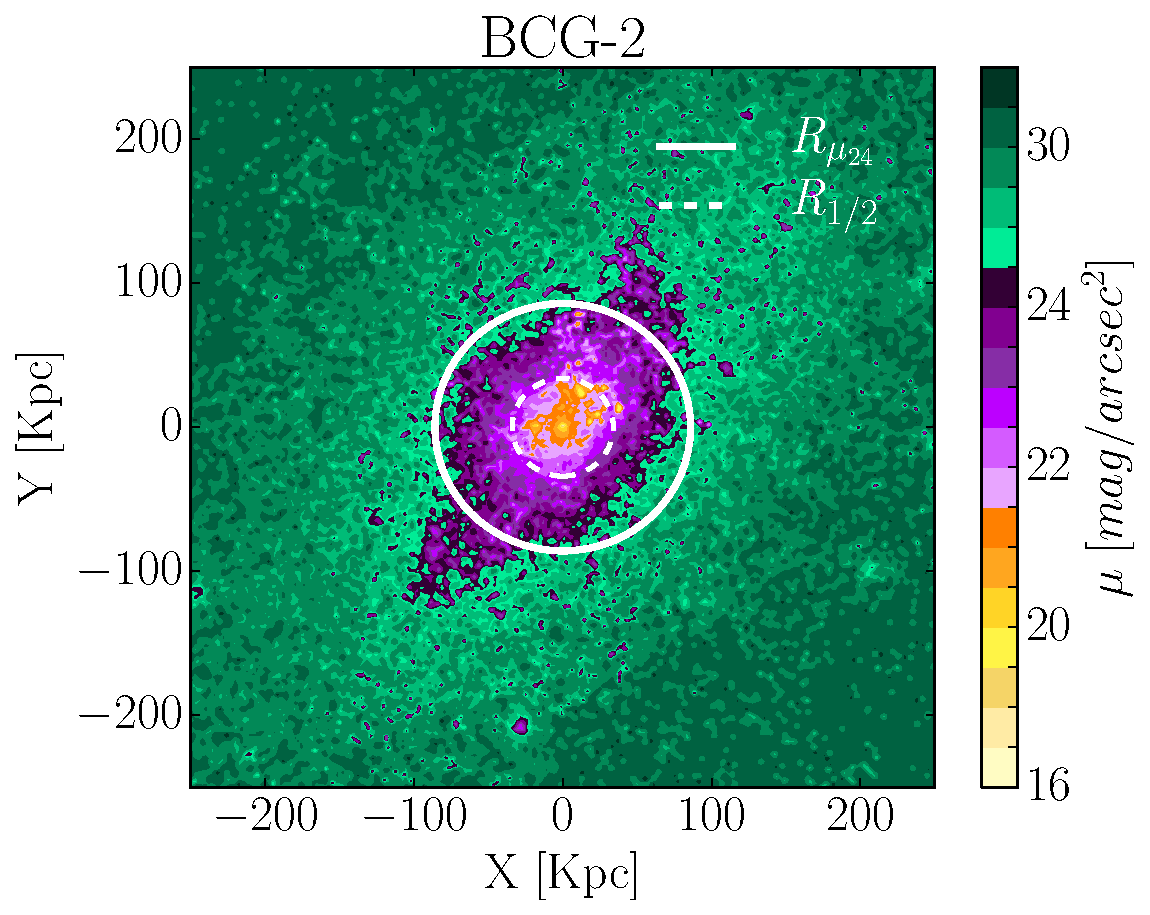
\includegraphics[height=8cm, width=9.0cm, trim={3.2cm 0cm 0cm 1.1cm},clip]{../al_final/LR/LR_minpot3_rmmax/nodust/grupo0/mu24/D2/091/maps_D2_aperturas.pdf}
\caption[csfagnmap]{}
\end{figure}



\begin{figure}[H]
 \centering
 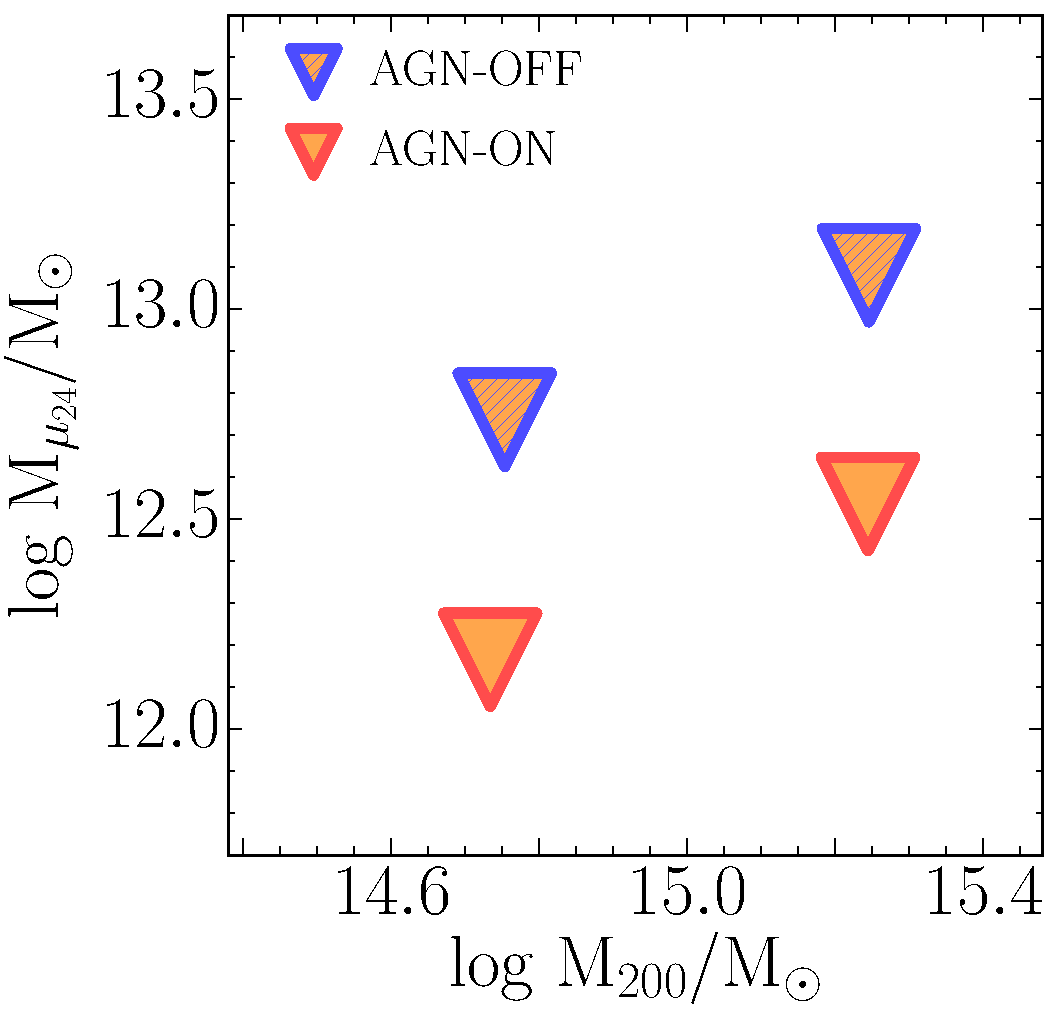
\includegraphics[height=8cm, width=9cm]{../al_final/LR/evolucion/relaciones/csf_agn.pdf}
\end{figure}

\begin{figure}[H]
 \centering
 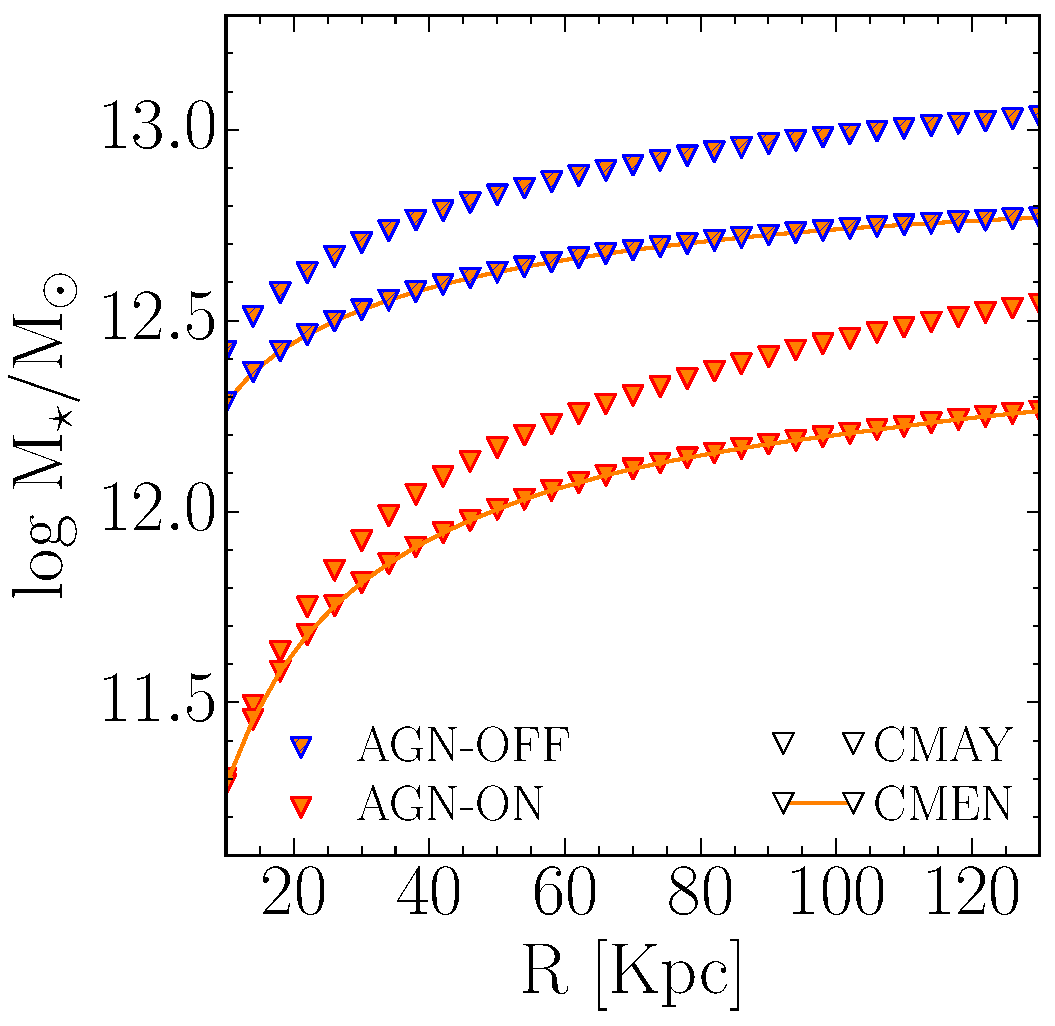
\includegraphics[height=8cm, width=9cm]{../al_final/LR/evolucion/relaciones/csf_agn_acumuladas.pdf}
 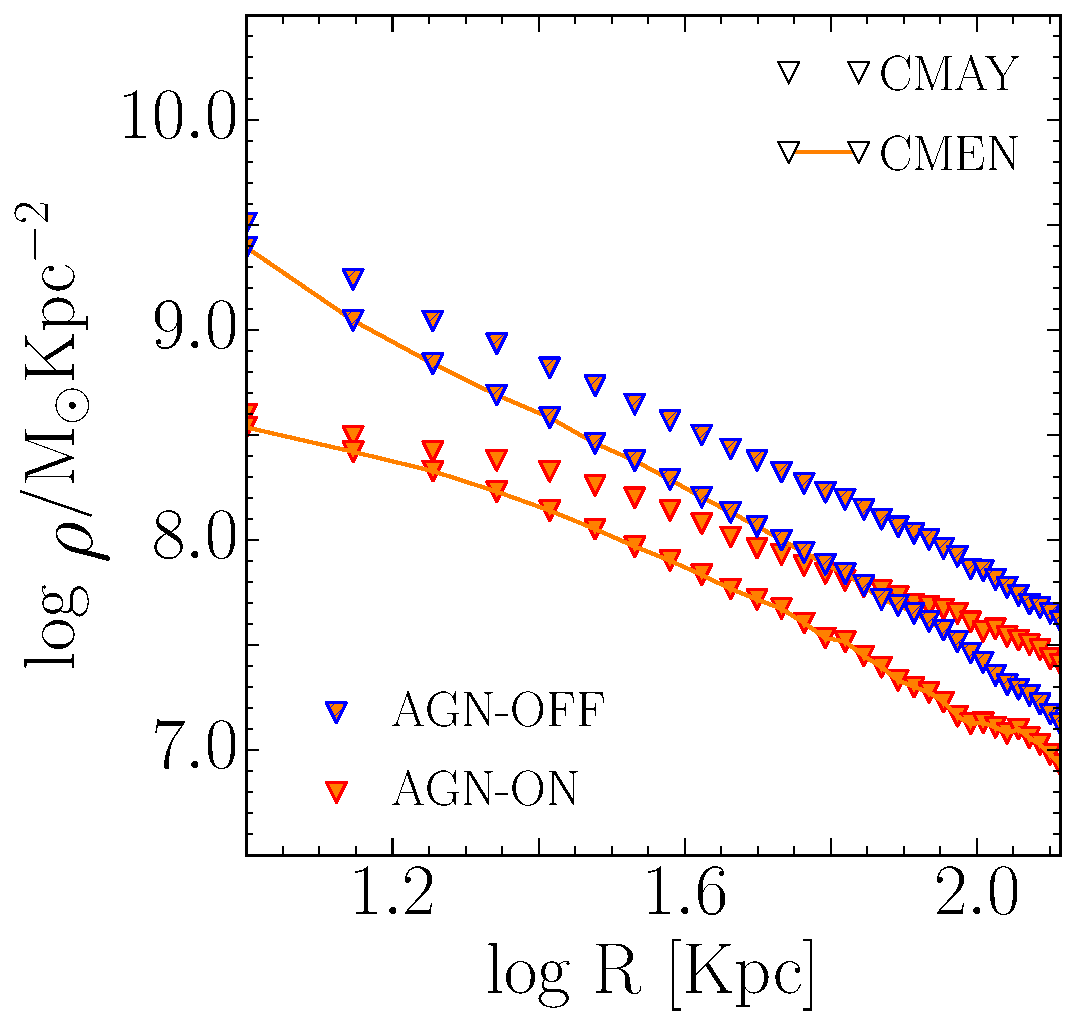
\includegraphics[height=8cm, width=9cm]{../al_final/LR/evolucion/relaciones/csf_agn_perfil_dens_masa_con_log.pdf}
\end{figure}


\section{Masas de la BCG en funci\'on de la apertura}

%la mas excentrica
\begin{figure}[H]
 \centering
 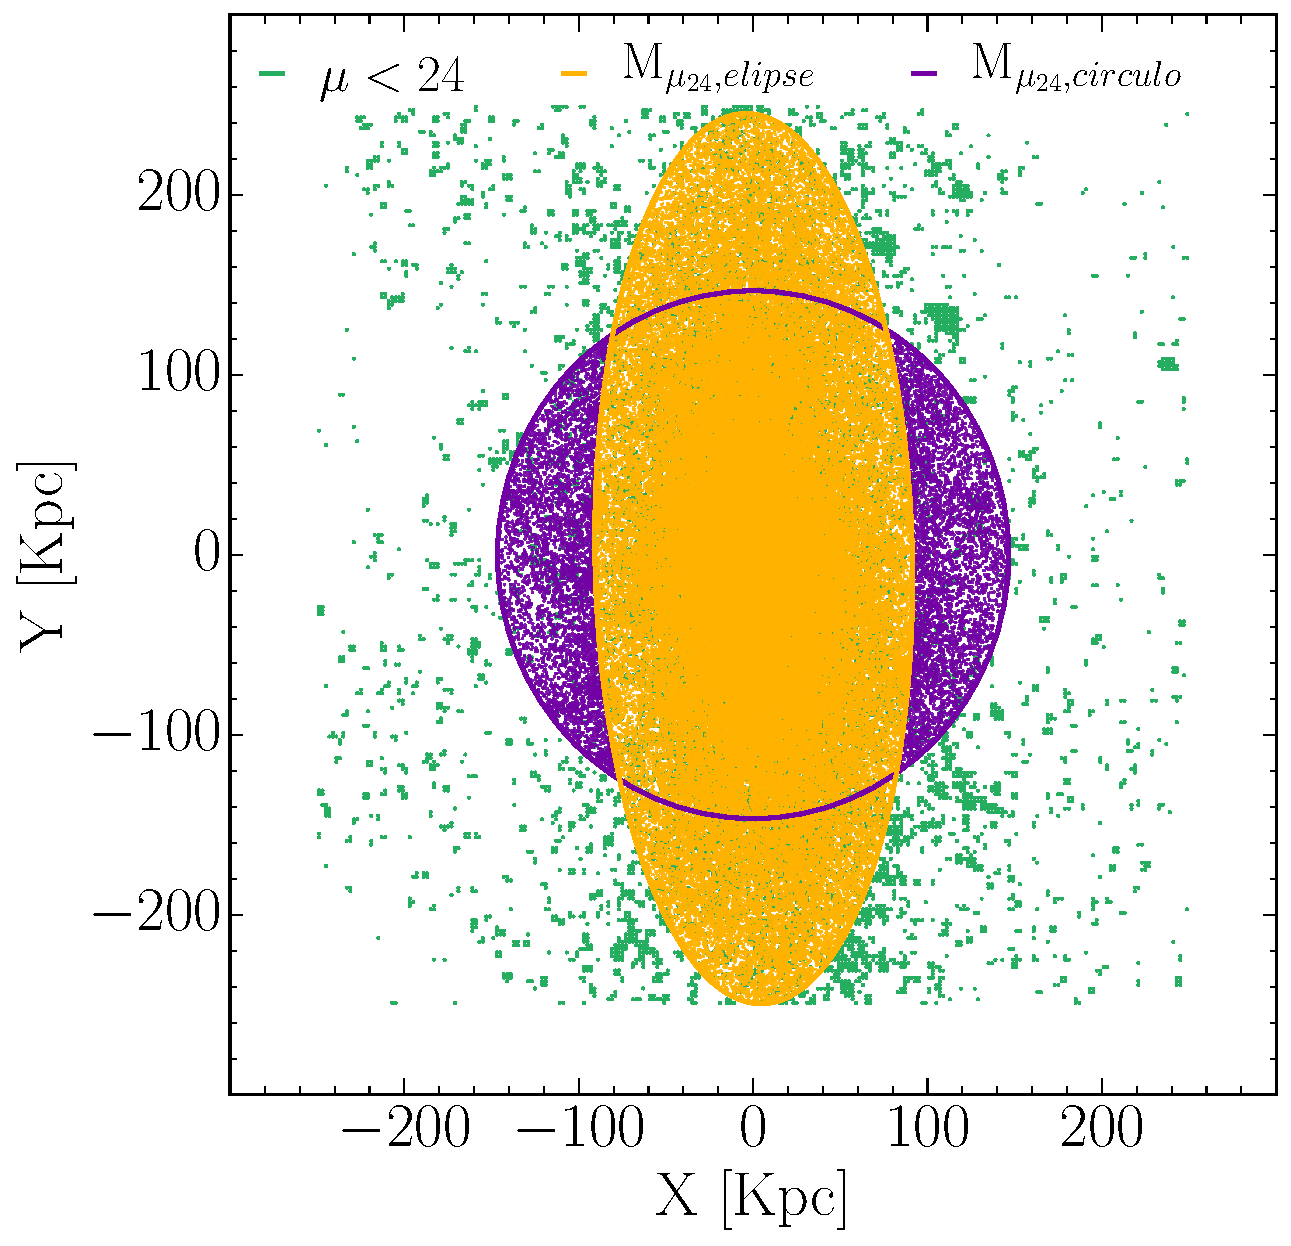
\includegraphics[height=9cm, width=9cm]{../al_final/plots/elipses/D22elipse-circ.pdf}
\end{figure}

\begin{figure}[H]
 \centering
 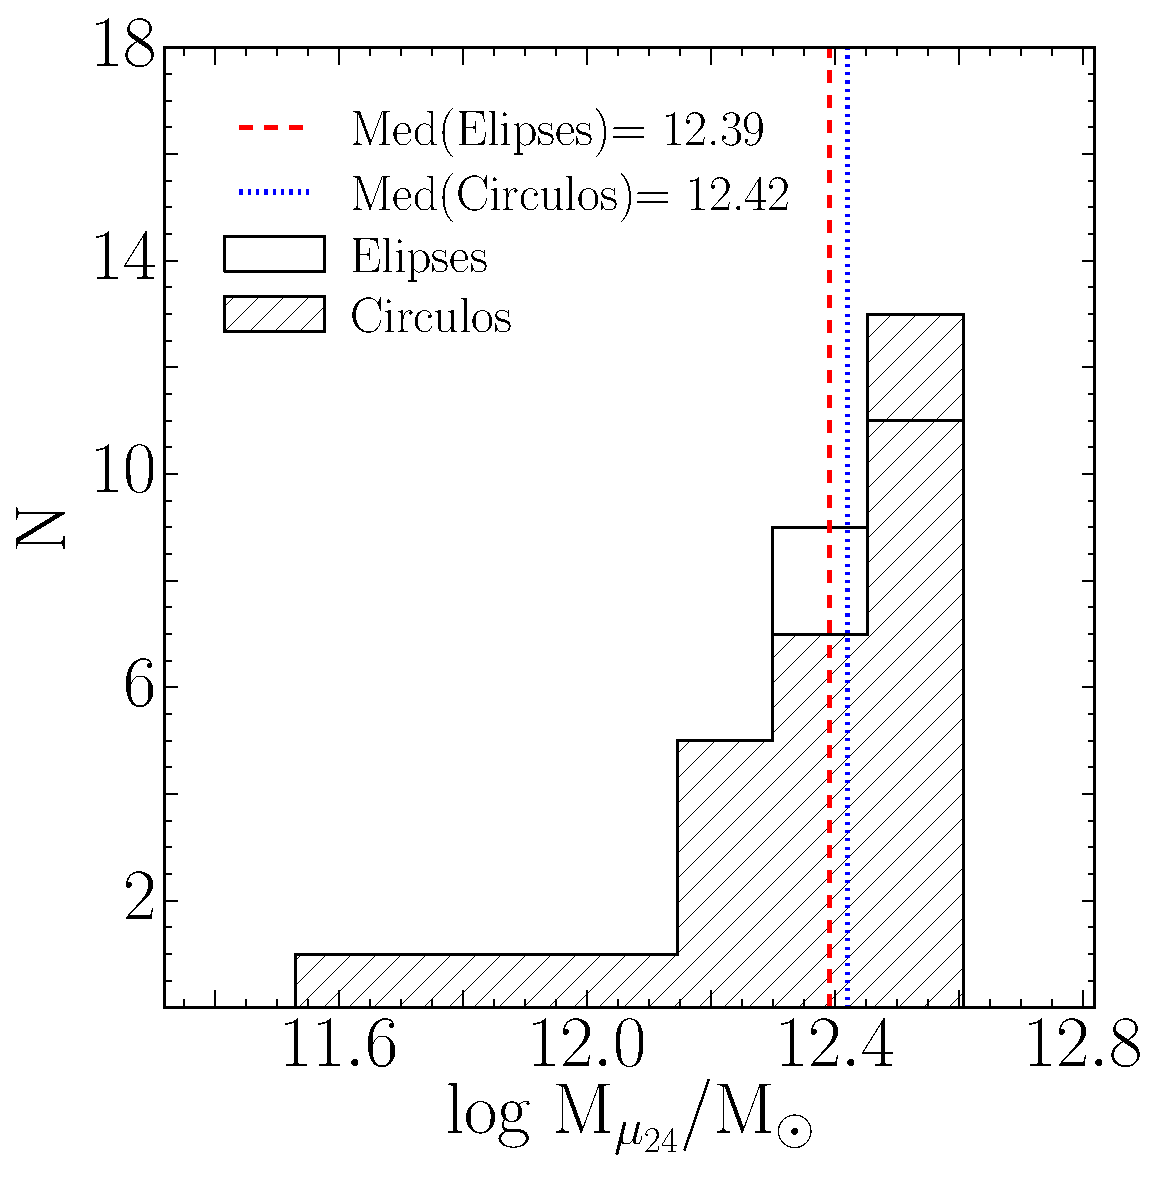
\includegraphics[height=9cm, width=9cm]{../al_final/LR/evolucion/histogramas/Mmu_elipse_vs_circ.pdf}
\end{figure}

\section{BCGs z=0}


\begin{tabular}{c c c c c}
\hspace*{-1cm} 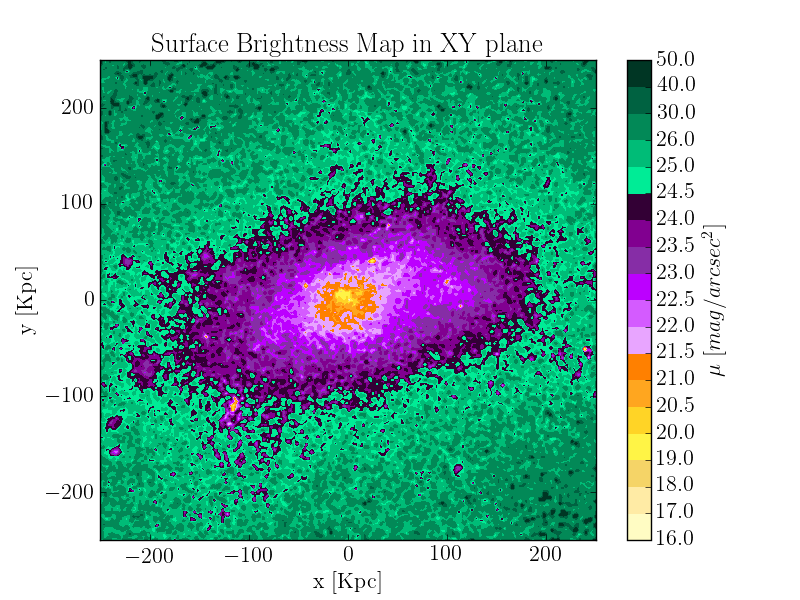
\includegraphics[height=4cm,width=4cm,trim={2.5cm 1.5cm 5cm 1.5cm},clip]{../pngs/D1.png}  & 
 \hspace*{-0.3cm}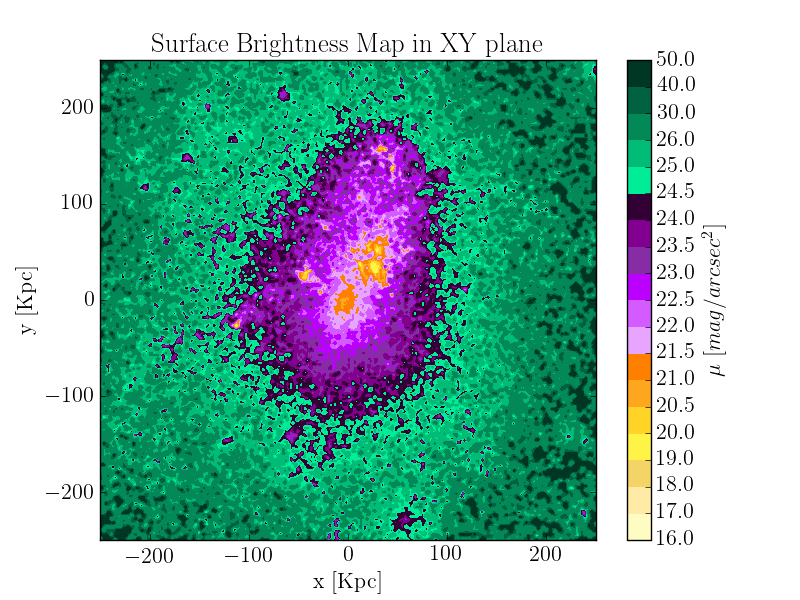
\includegraphics[height=4cm,width=4cm,trim={2.5cm 1.5cm 5cm 1.5cm},clip]{../pngs/D6.png}  & 
 \hspace*{-0.3cm}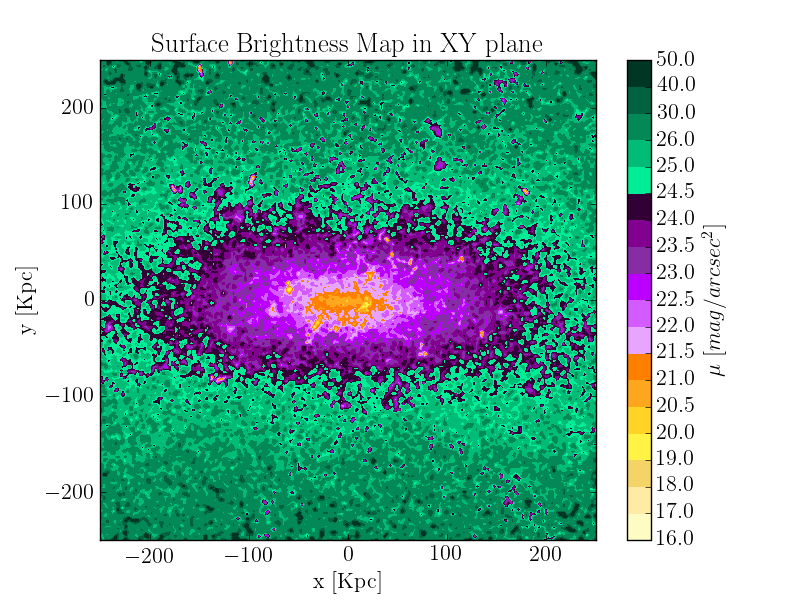
\includegraphics[height=4cm,width=4cm,trim={2.5cm 1.5cm 5cm 1.5cm},clip]{../pngs/D7.png}  & 
 \hspace*{-0.3cm}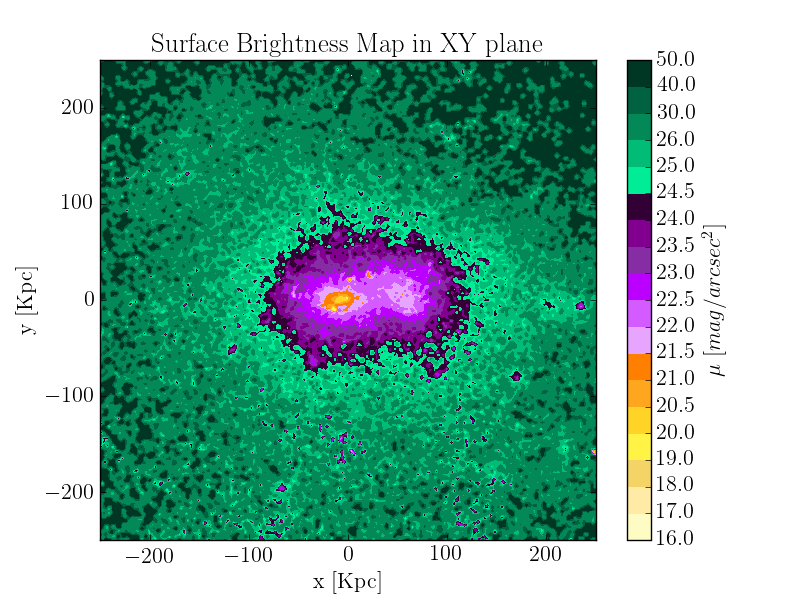
\includegraphics[height=4cm,width=4cm,trim={2.5cm 1.5cm 5cm 1.5cm},clip]{../pngs/D8.png}  & 
  \hspace*{-0.3cm}\multirow{6}{*}
  {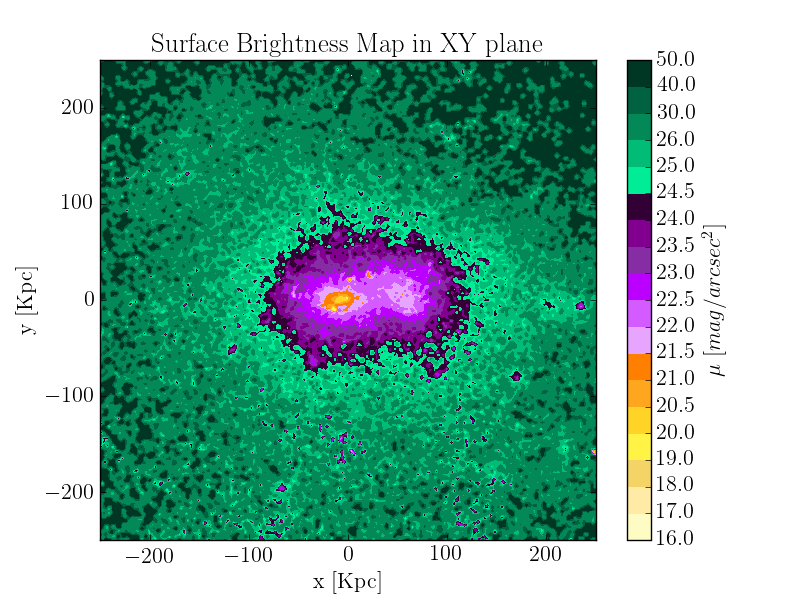
\includegraphics[height=15cm,width=3cm,trim={15.5cm 1.cm 0cm 1.cm},clip]{../pngs/D8.png}}
 \\

 \hspace*{-1cm}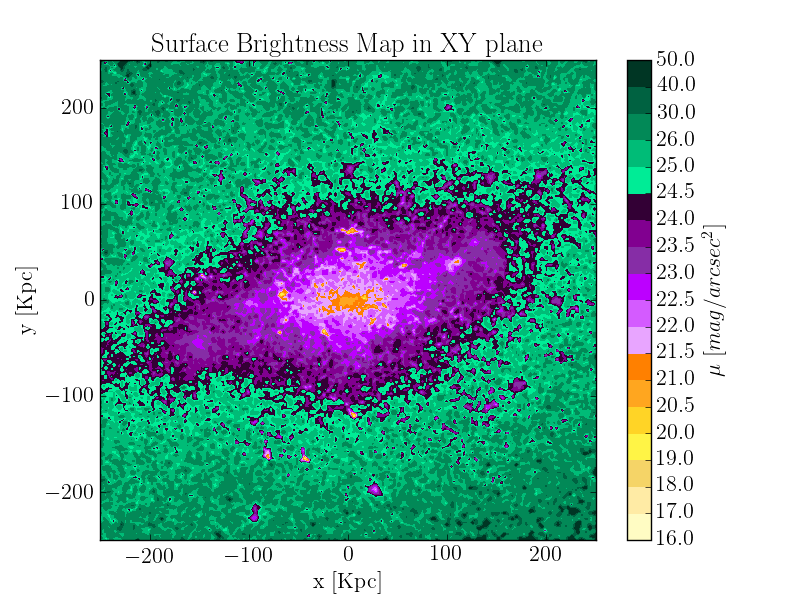
\includegraphics[height=4cm,width=4cm,trim={2.5cm 1.5cm 5cm 1.5cm},clip]{../pngs/D10.png}  & 
 \hspace*{-.3cm}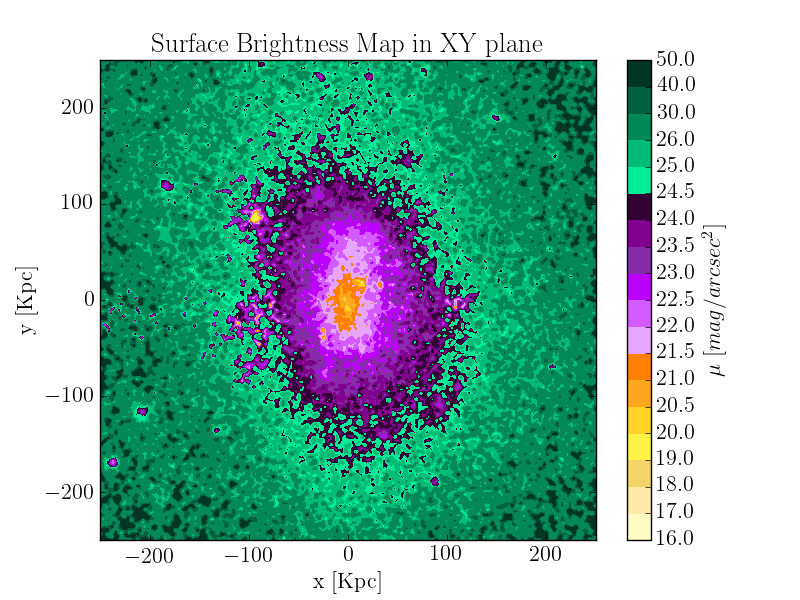
\includegraphics[height=4cm,width=4cm,trim={2.5cm 1.5cm 5cm 1.5cm},clip]{../pngs/D11.png}  & 
 \hspace*{-.3cm}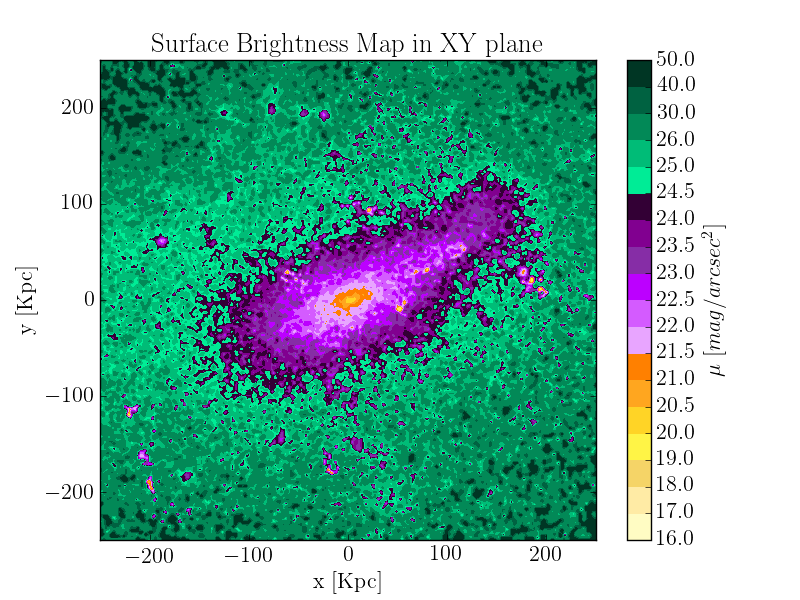
\includegraphics[height=4cm,width=4cm,trim={2.5cm 1.5cm 5cm 1.5cm},clip]{../pngs/D12.png}  & 
 \hspace*{-.3cm}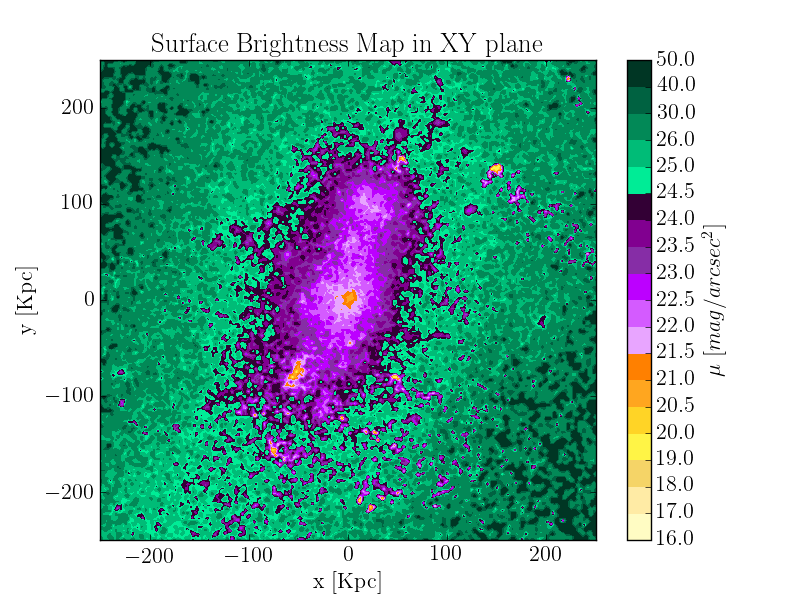
\includegraphics[height=4cm,width=4cm,trim={2.5cm 1.5cm 5cm 1.5cm},clip]{../pngs/D13.png}  &
 \\

 \hspace*{-1cm}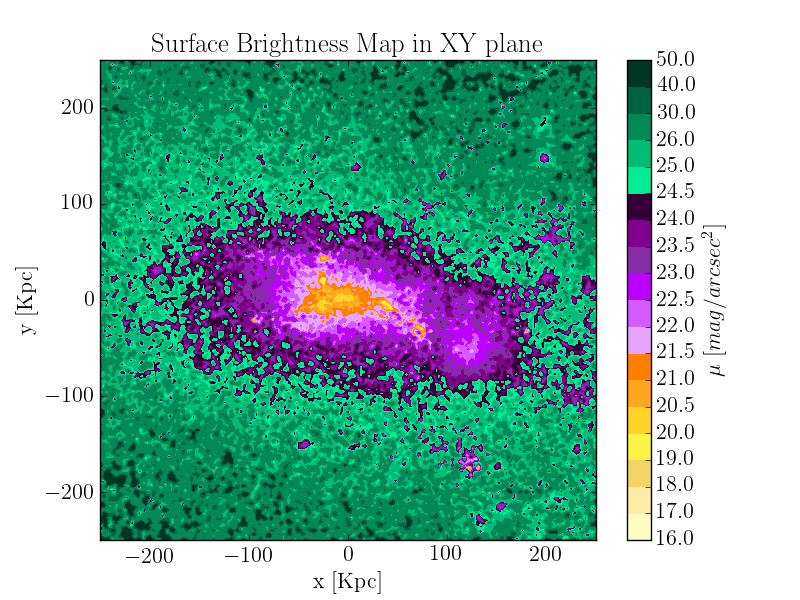
\includegraphics[height=4cm,width=4cm,trim={2.5cm 1.5cm 5cm 1.5cm},clip]{../pngs/D14.png}  & 
 \hspace*{-.3cm}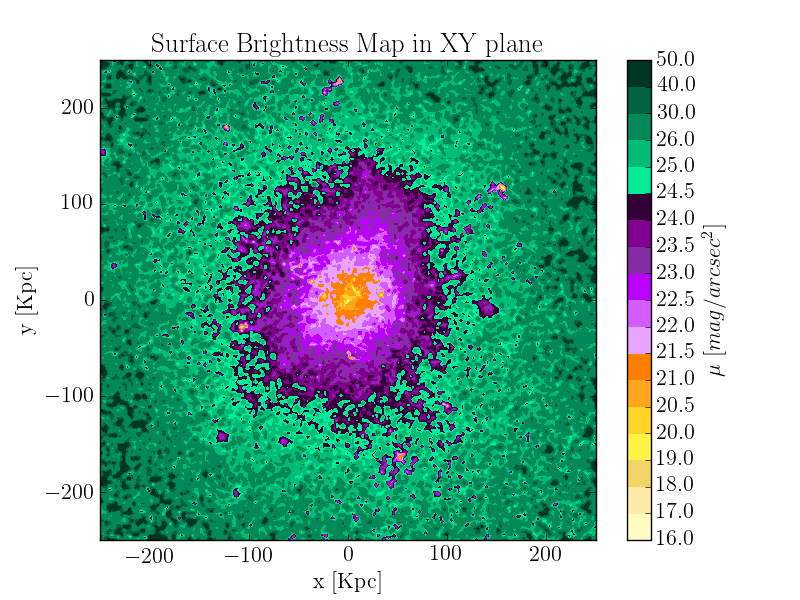
\includegraphics[height=4cm,width=4cm,trim={2.5cm 1.5cm 5cm 1.5cm},clip]{../pngs/D15.png}  & 
 \hspace*{-.3cm}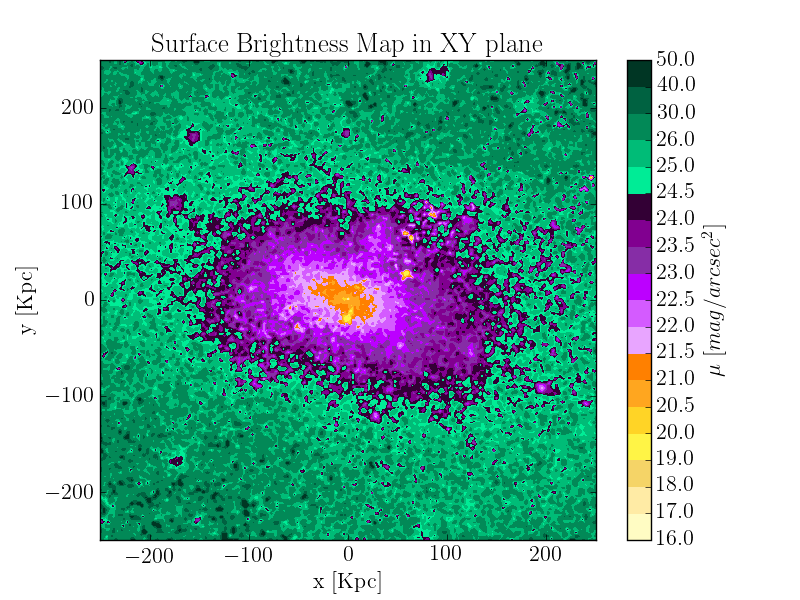
\includegraphics[height=4cm,width=4cm,trim={2.5cm 1.5cm 5cm 1.5cm},clip]{../pngs/D16.png}  & 
 \hspace*{-.3cm}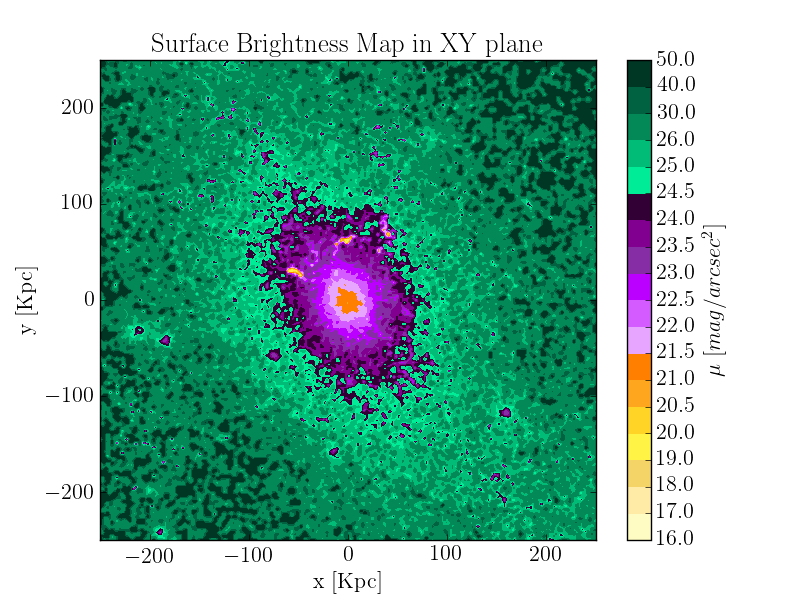
\includegraphics[height=4cm,width=4cm,trim={2.5cm 1.5cm 5cm 1.5cm},clip]{../pngs/D17.png}  &
 \\ 

 \hspace*{-1cm}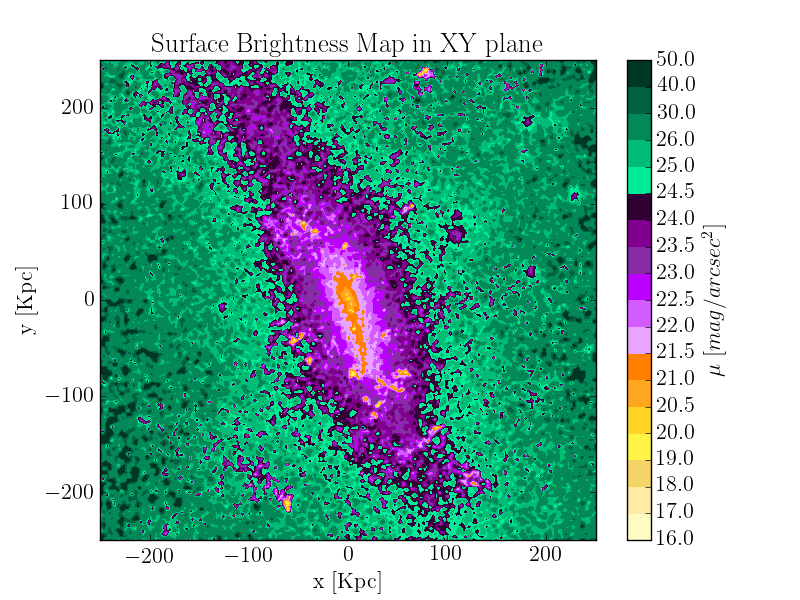
\includegraphics[height=4cm,width=4cm,trim={2.5cm 1.5cm 5cm 1.5cm},clip]{../pngs/D18.png}  & 
 \hspace*{-.3cm}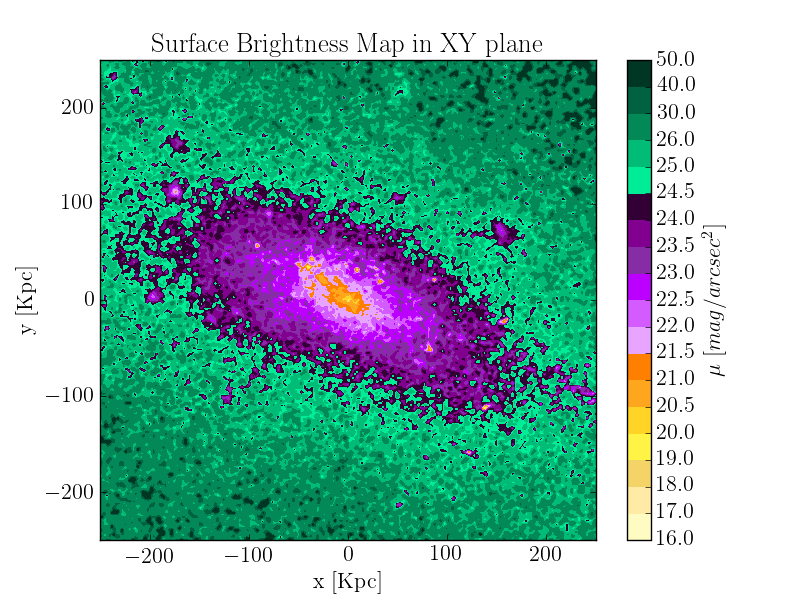
\includegraphics[height=4cm,width=4cm,trim={2.5cm 1.5cm 5cm 1.5cm},clip]{../pngs/D19.png}  & 
 \hspace*{-.3cm}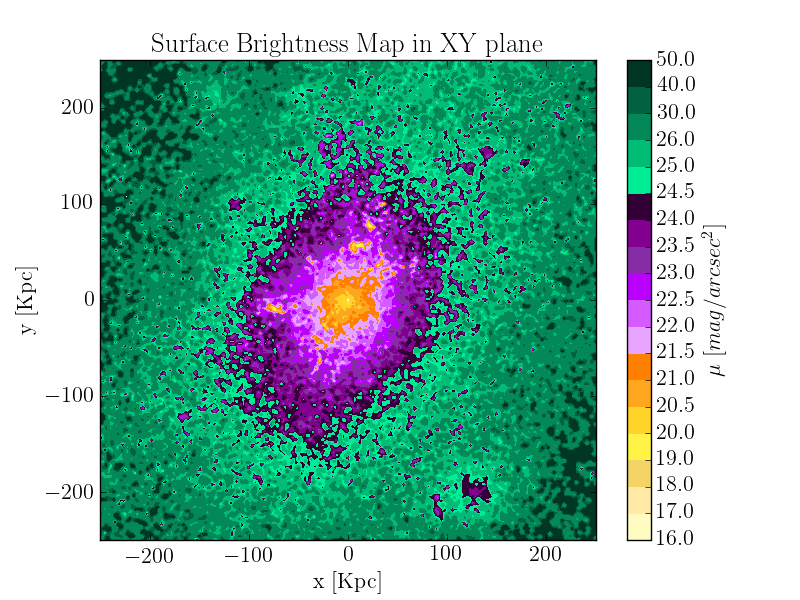
\includegraphics[height=4cm,width=4cm,trim={2.5cm 1.5cm 5cm 1.5cm},clip]{../pngs/D20.png}  & 
 \hspace*{-.3cm}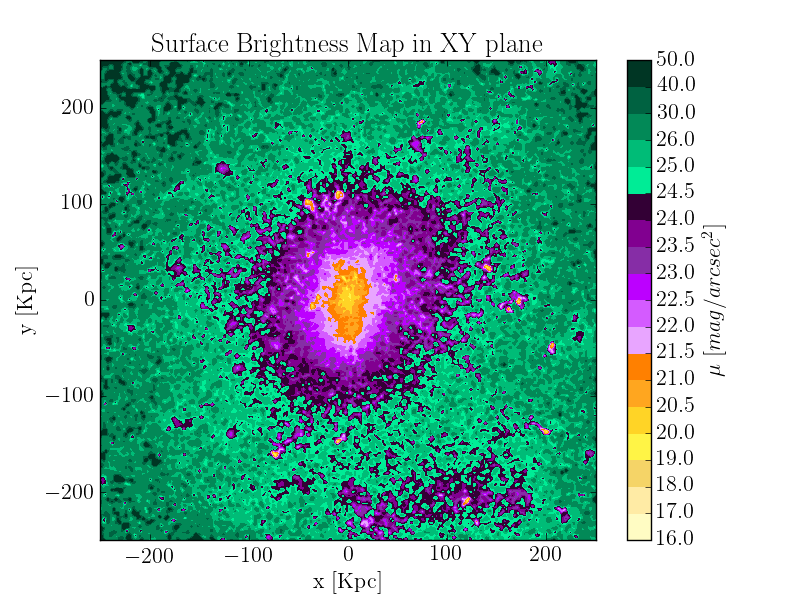
\includegraphics[height=4cm,width=4cm,trim={2.5cm 1.5cm 5cm 1.5cm},clip]{../pngs/D21.png}  &
 \\ 

 \hspace*{-1cm}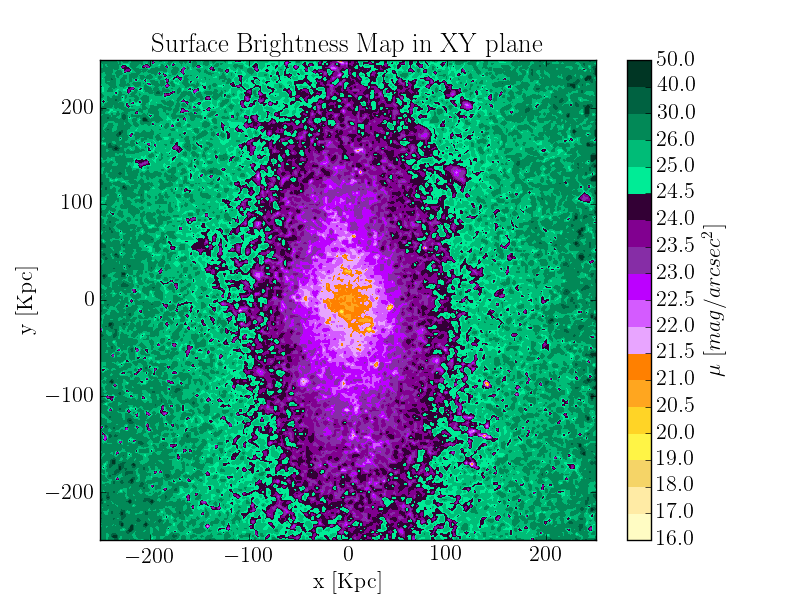
\includegraphics[height=4cm,width=4cm,trim={2.5cm 1.5cm 5cm 1.5cm},clip]{../pngs/D22.png}  & 
 \hspace*{-.3cm}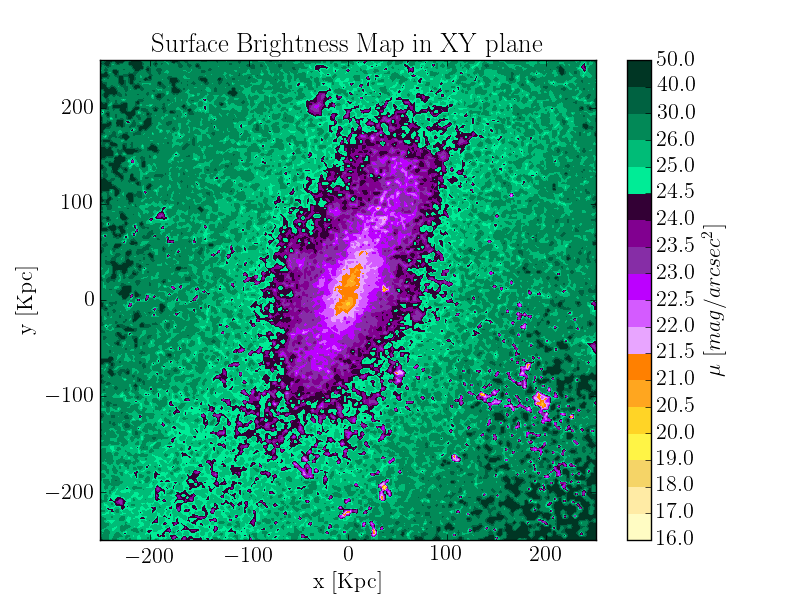
\includegraphics[height=4cm,width=4cm,trim={2.5cm 1.5cm 5cm 1.5cm},clip]{../pngs/D23.png}  & 
 \hspace*{-.3cm}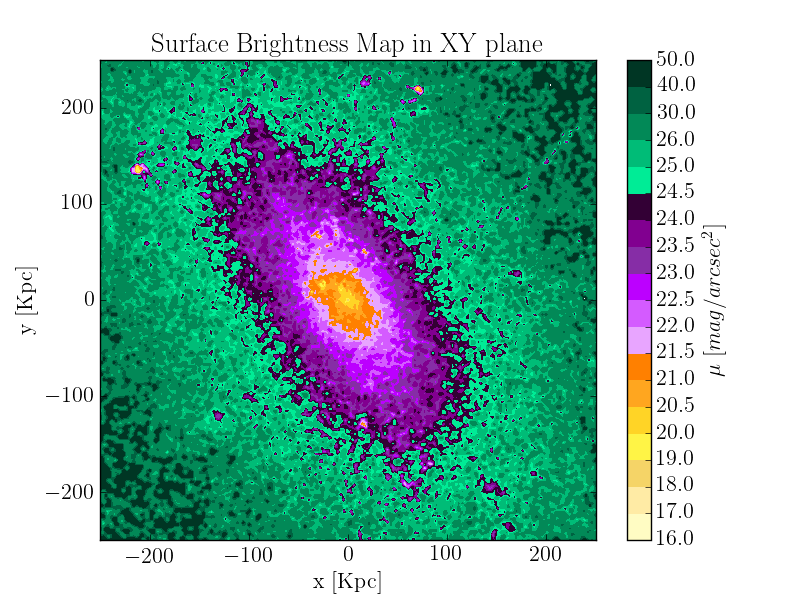
\includegraphics[height=4cm,width=4cm,trim={2.5cm 1.5cm 5cm 1.5cm},clip]{../pngs/D24.png}  & 
 \hspace*{-.3cm}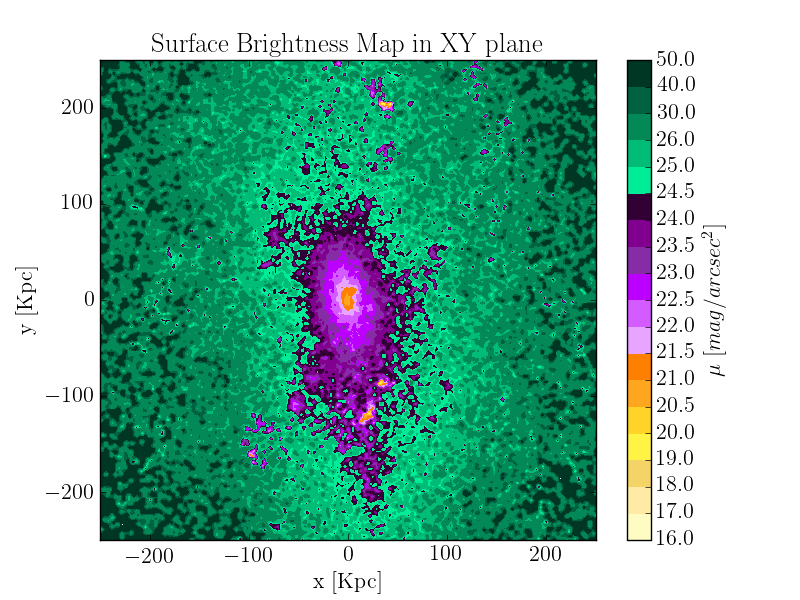
\includegraphics[height=4cm,width=4cm,trim={2.5cm 1.5cm 5cm 1.5cm},clip]{../pngs/D25.png}  &
 \\ 

 \hspace*{-1cm}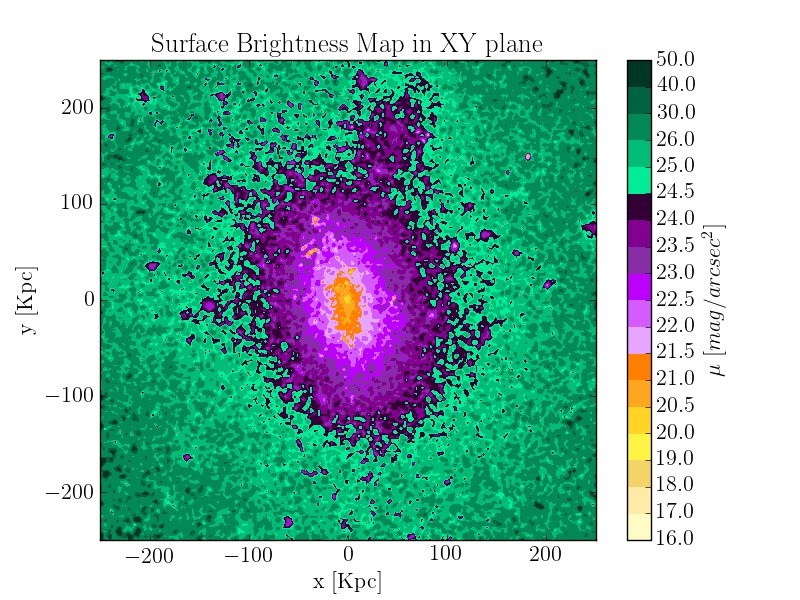
\includegraphics[height=4cm,width=4cm,trim={2.5cm 1.5cm 5cm 1.5cm},clip]{../pngs/D26.png}  & 
 \hspace*{-.3cm}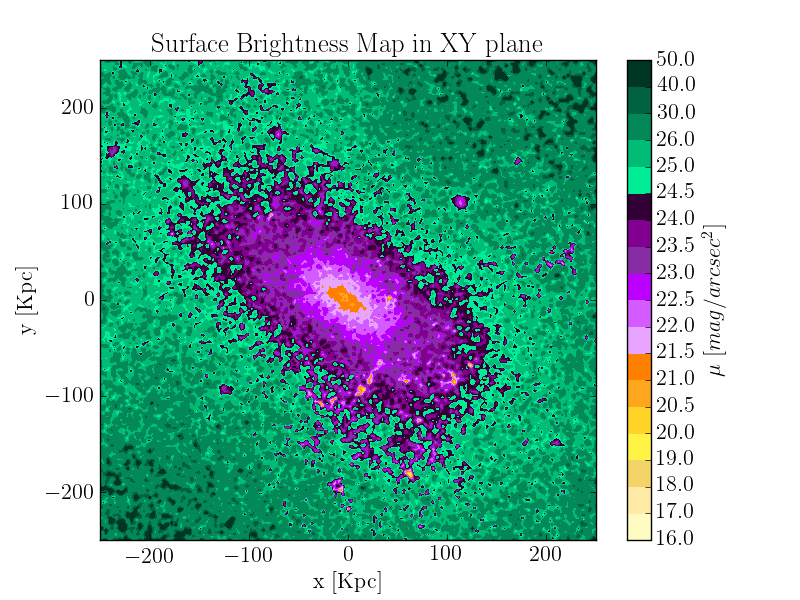
\includegraphics[height=4cm,width=4cm,trim={2.5cm 1.5cm 5cm 1.5cm},clip]{../pngs/D27.png}  & 
 \hspace*{-.3cm}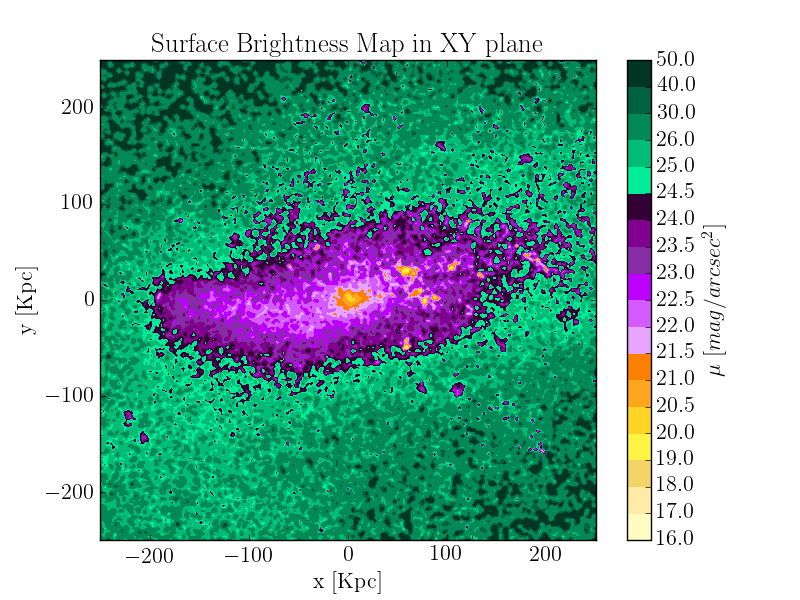
\includegraphics[height=4cm,width=4cm,trim={2.5cm 1.5cm 5cm 1.5cm},clip]{../pngs/D28.png}  & 
 \hspace*{-.3cm}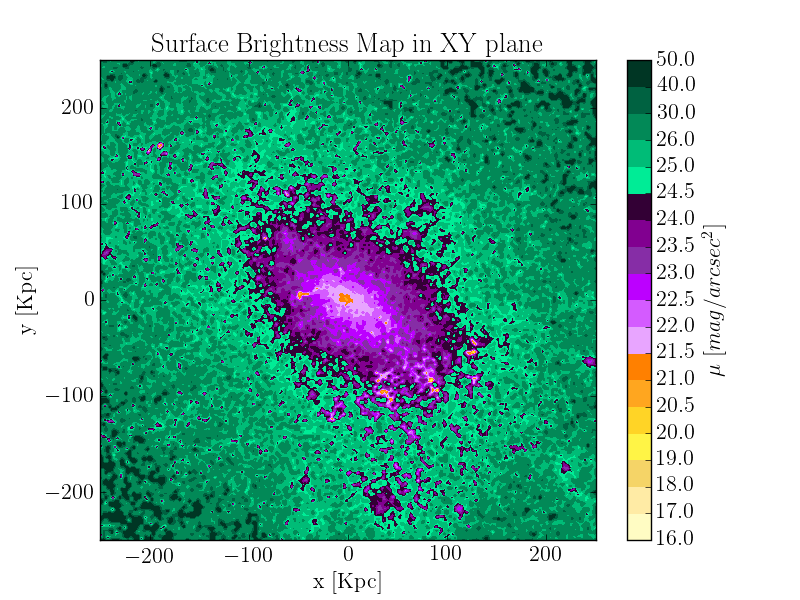
\includegraphics[height=4cm,width=4cm,trim={2.5cm 1.5cm 5cm 1.5cm},clip]{../pngs/D29.png}  &
 \\
 
\end{tabular}


\begin{figure}[H]
 \centering
 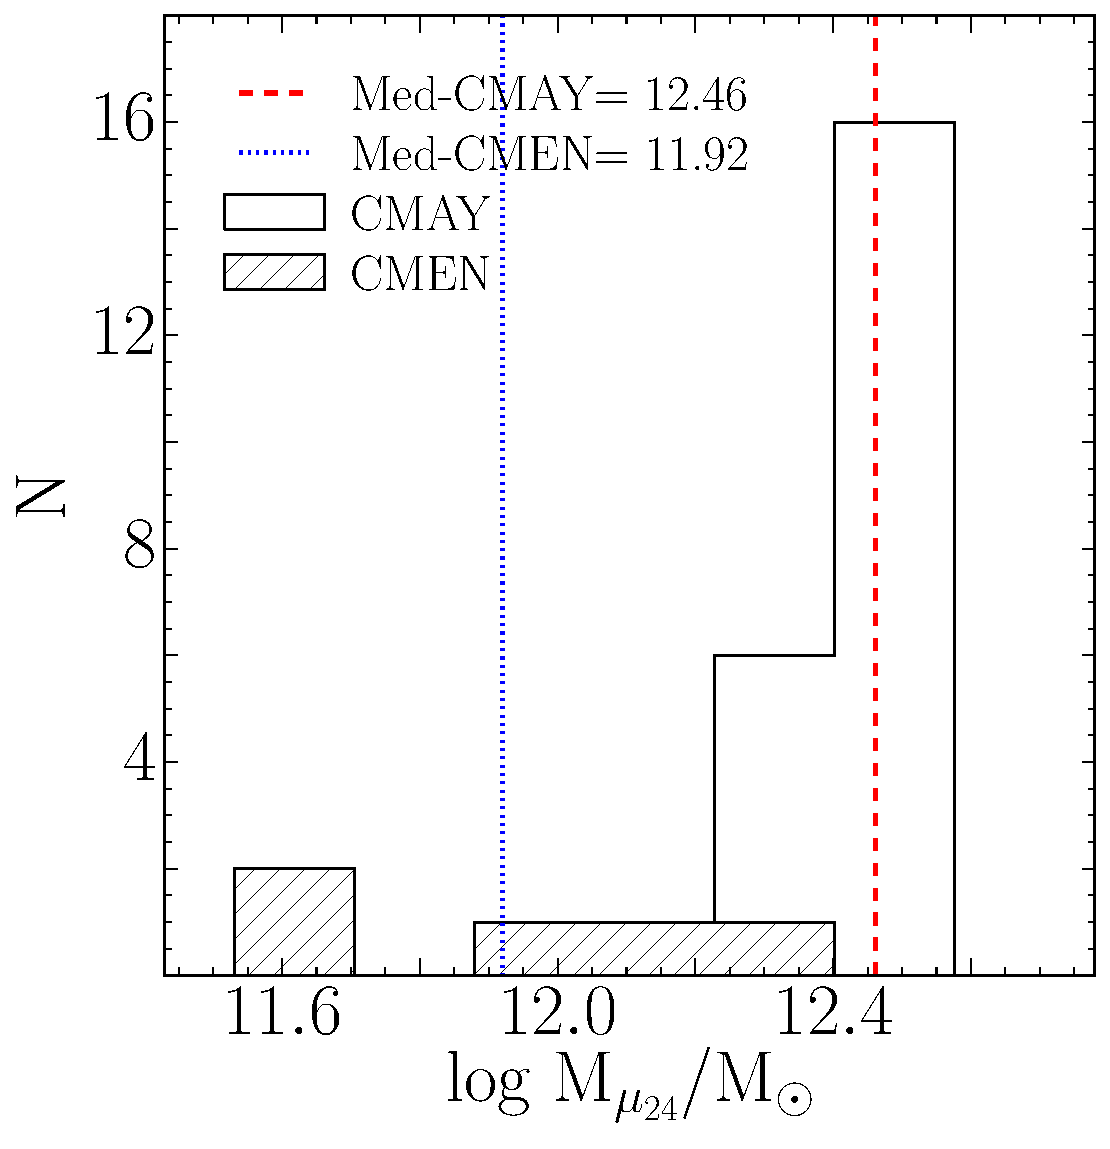
\includegraphics[height=9cm, width=9cm]{../al_final/LR/evolucion/histogramas/Mmu_grandes_chicasz0.pdf}
\end{figure}
\begin{figure}[H]
 \centering
 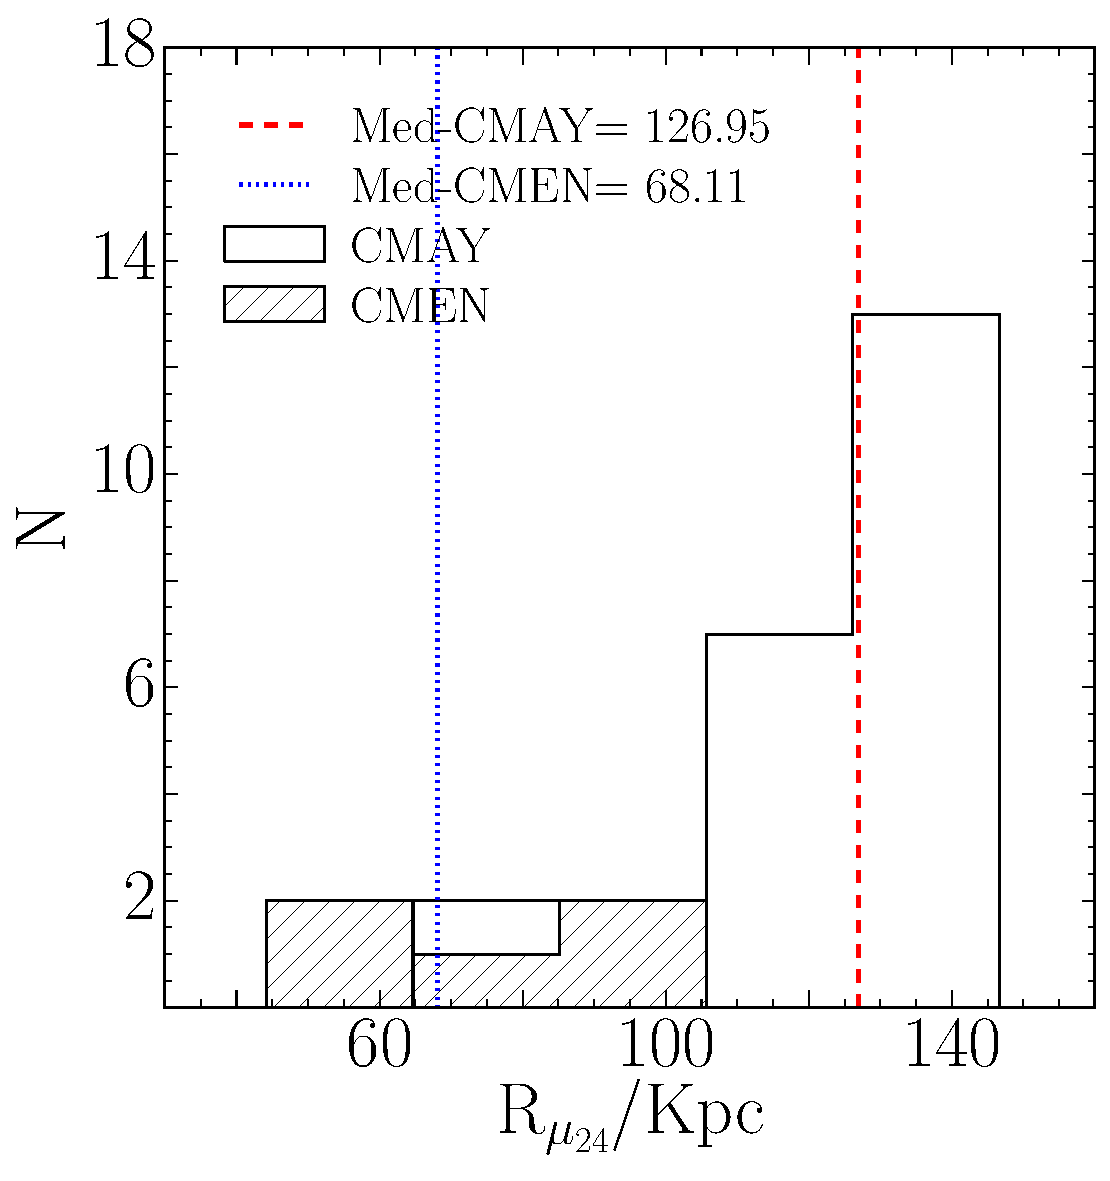
\includegraphics[height=9cm, width=9cm]{../al_final/LR/evolucion/histogramas/R24_grandes_chicasz0.pdf}
\end{figure}
\begin{figure}[H]
 \centering
 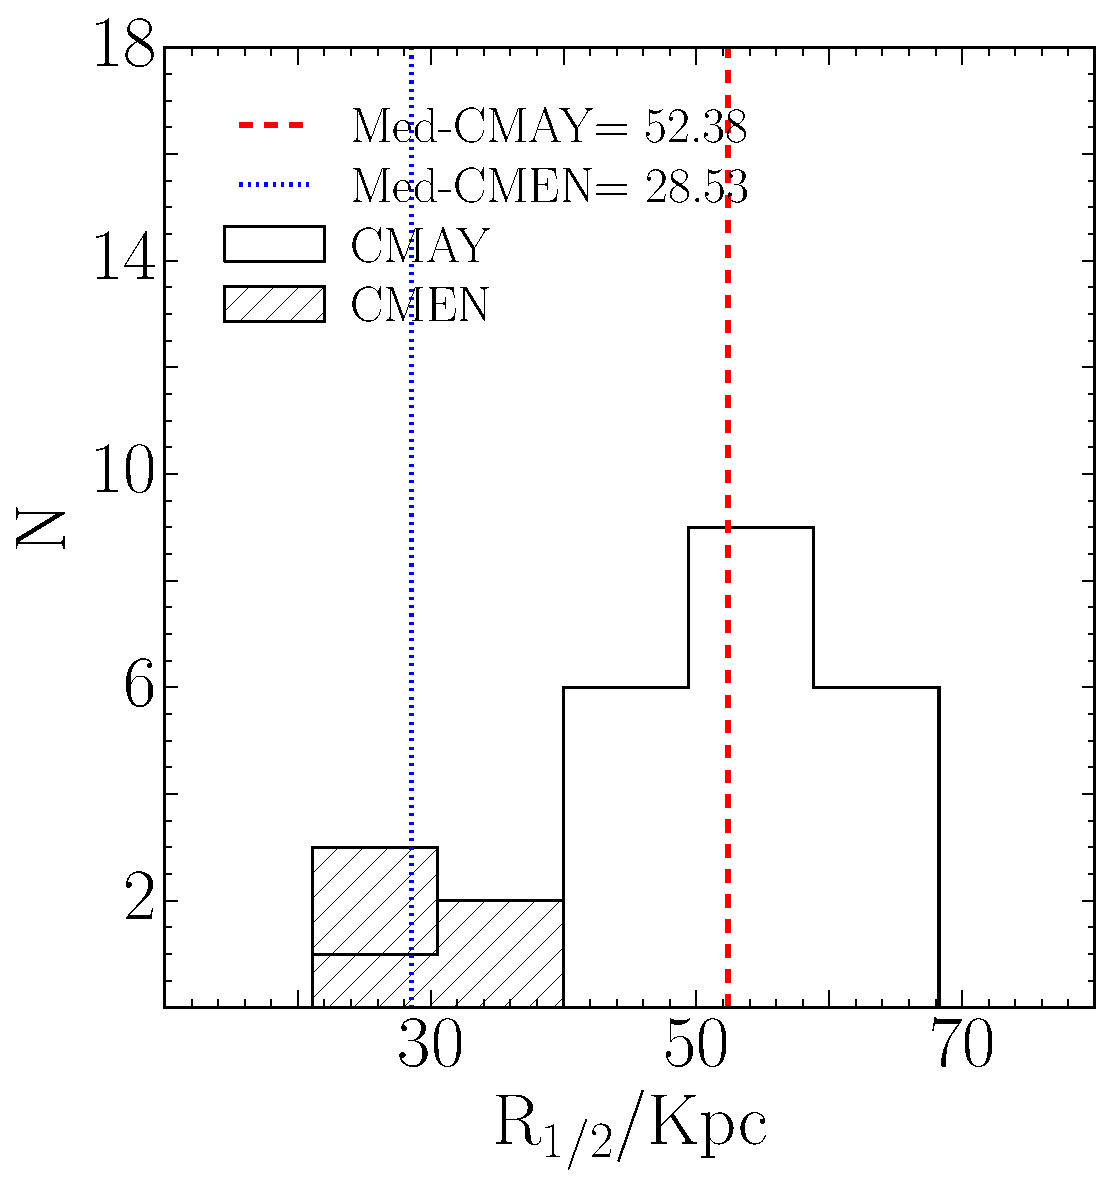
\includegraphics[height=9cm, width=9cm]{../al_final/LR/evolucion/histogramas/R50_grandes_chicasz0.pdf}
\end{figure}



\section{Relaciones Masa-Masa C\'umulo}

\begin{figure}[H]
 \centering
 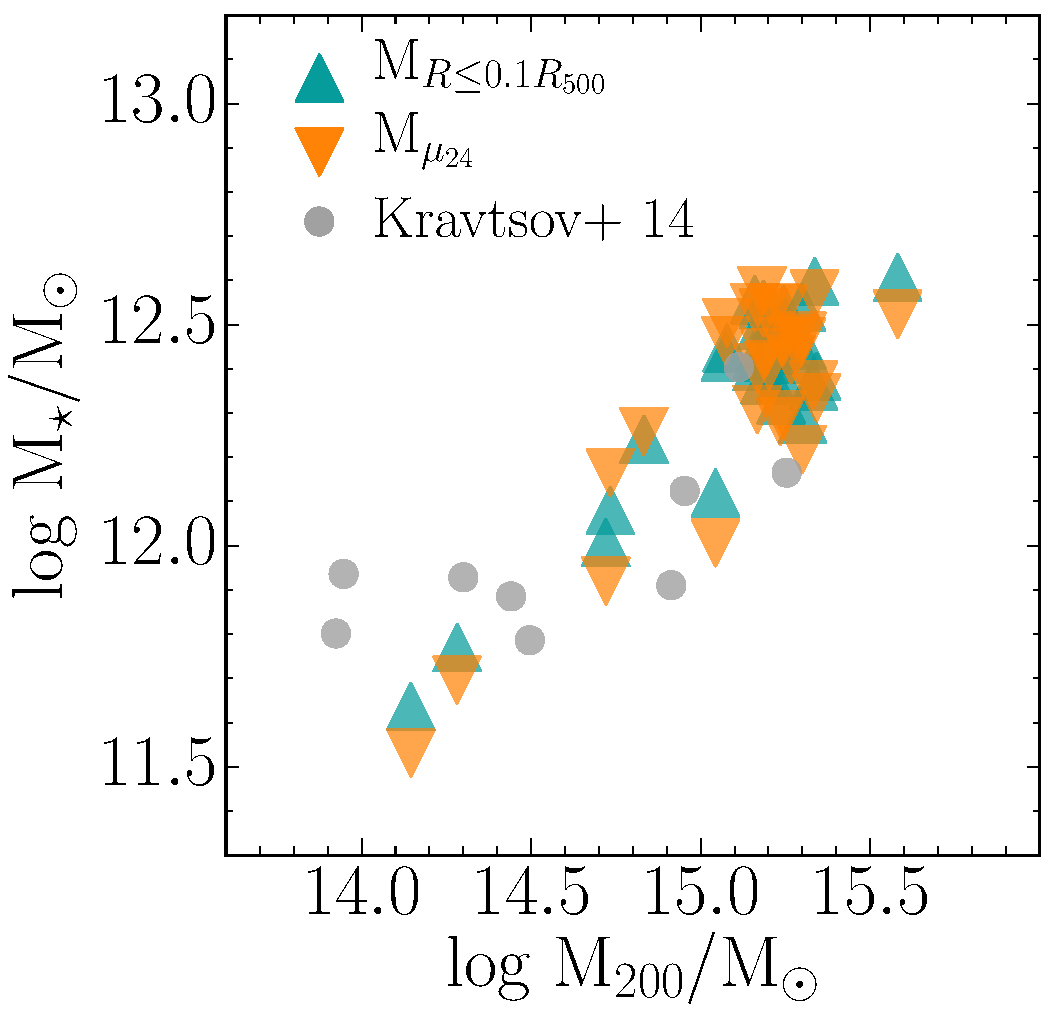
\includegraphics[height=9cm, width=10cm]{../al_final/LR/evolucion/relaciones/mtotales.pdf}
\end{figure}

\begin{figure}[H]
 \centering
 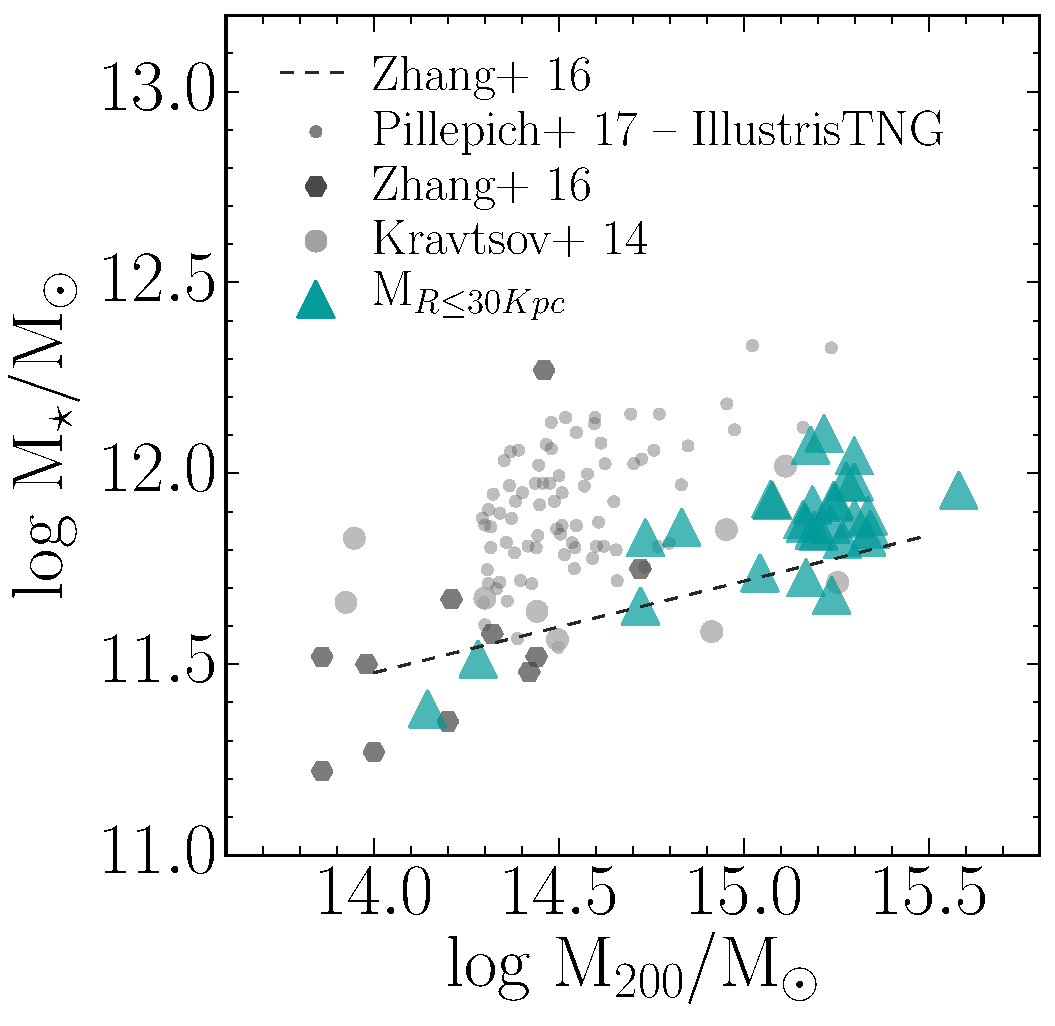
\includegraphics[height=9cm, width=10cm]{../al_final/LR/evolucion/relaciones/M302D_vs_M200.pdf}
\end{figure}

\begin{figure}[H]
 \centering
 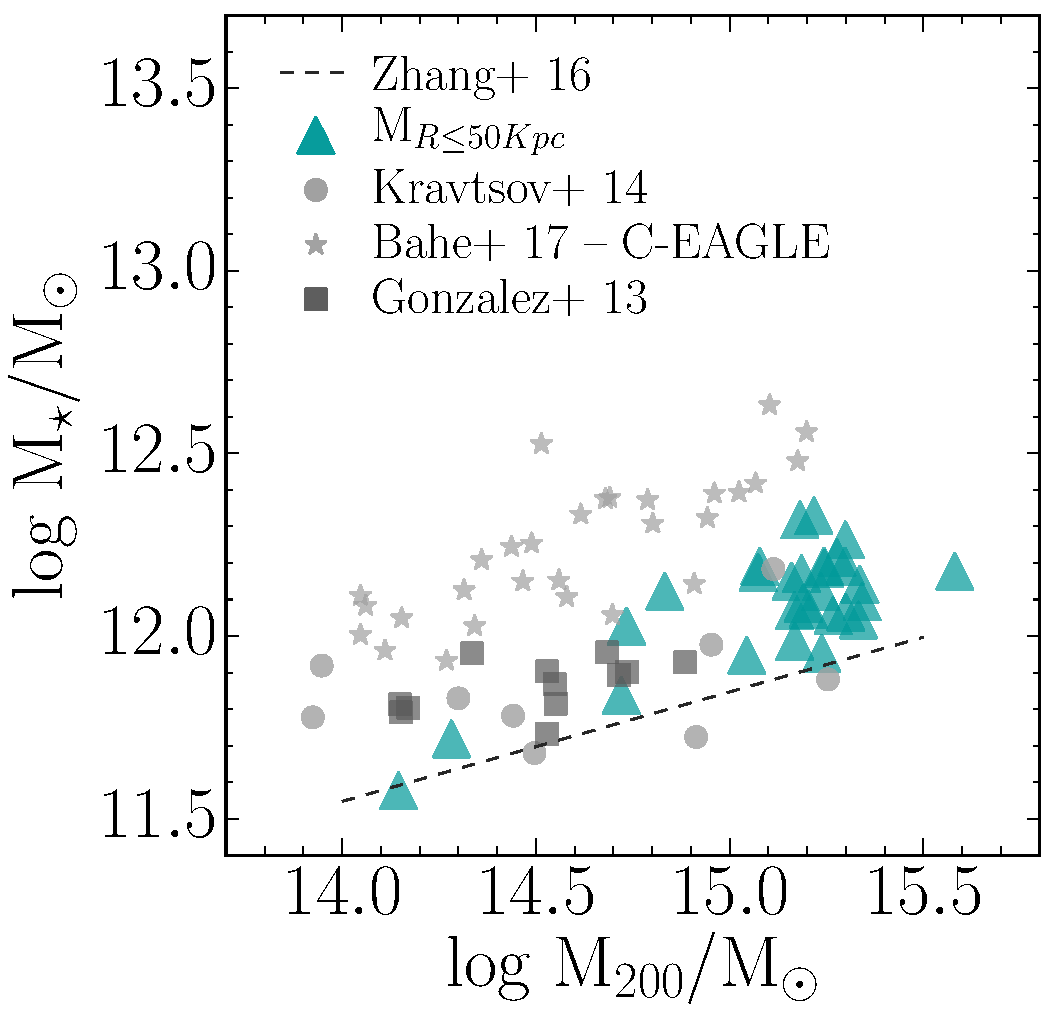
\includegraphics[height=9cm, width=10cm]{../al_final/LR/evolucion/relaciones/M502D_vs_M200.pdf}
\end{figure}



\section{Masas de las BCGs a distintos z}
\label{sec:zeta0}



\begin{figure}[H]
\centering
\hspace*{-1.5cm}
 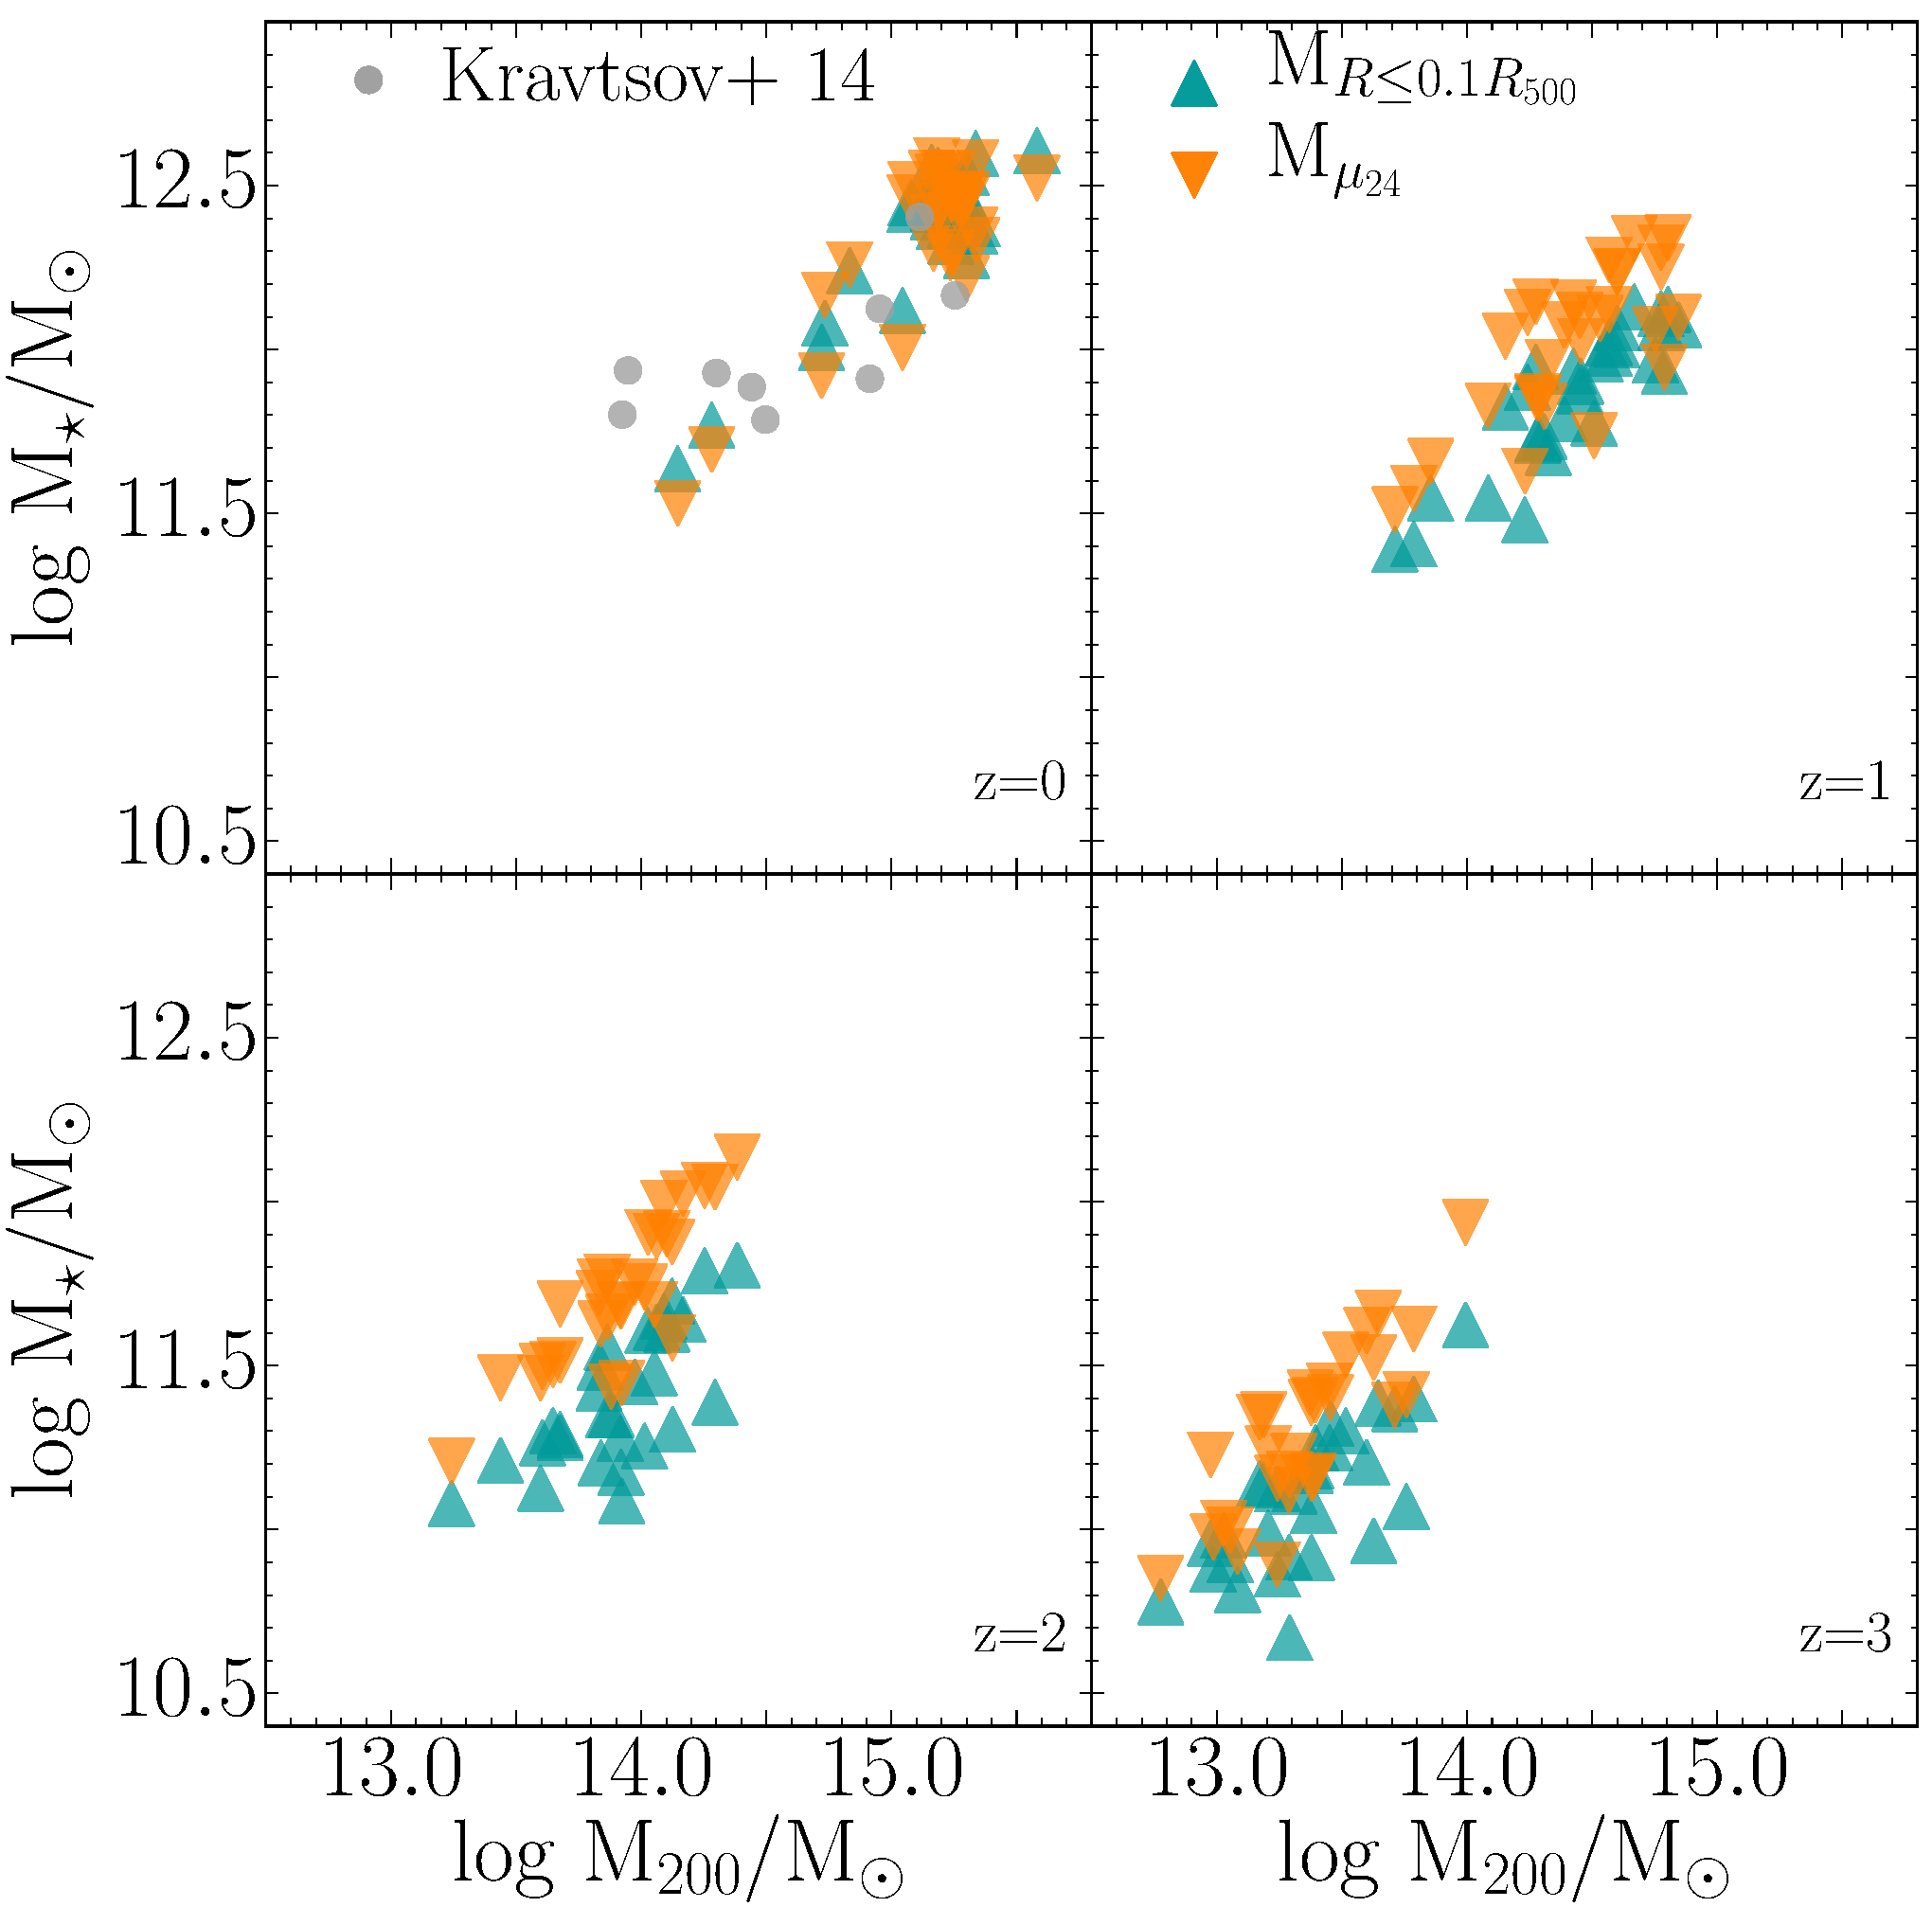
\includegraphics[height=12cm, width=13cm]{../al_final/LR/evolucion/relaciones/muvs10r.pdf}
\end{figure}

\begin{figure}[H]
\centering
\hspace*{-1cm}
 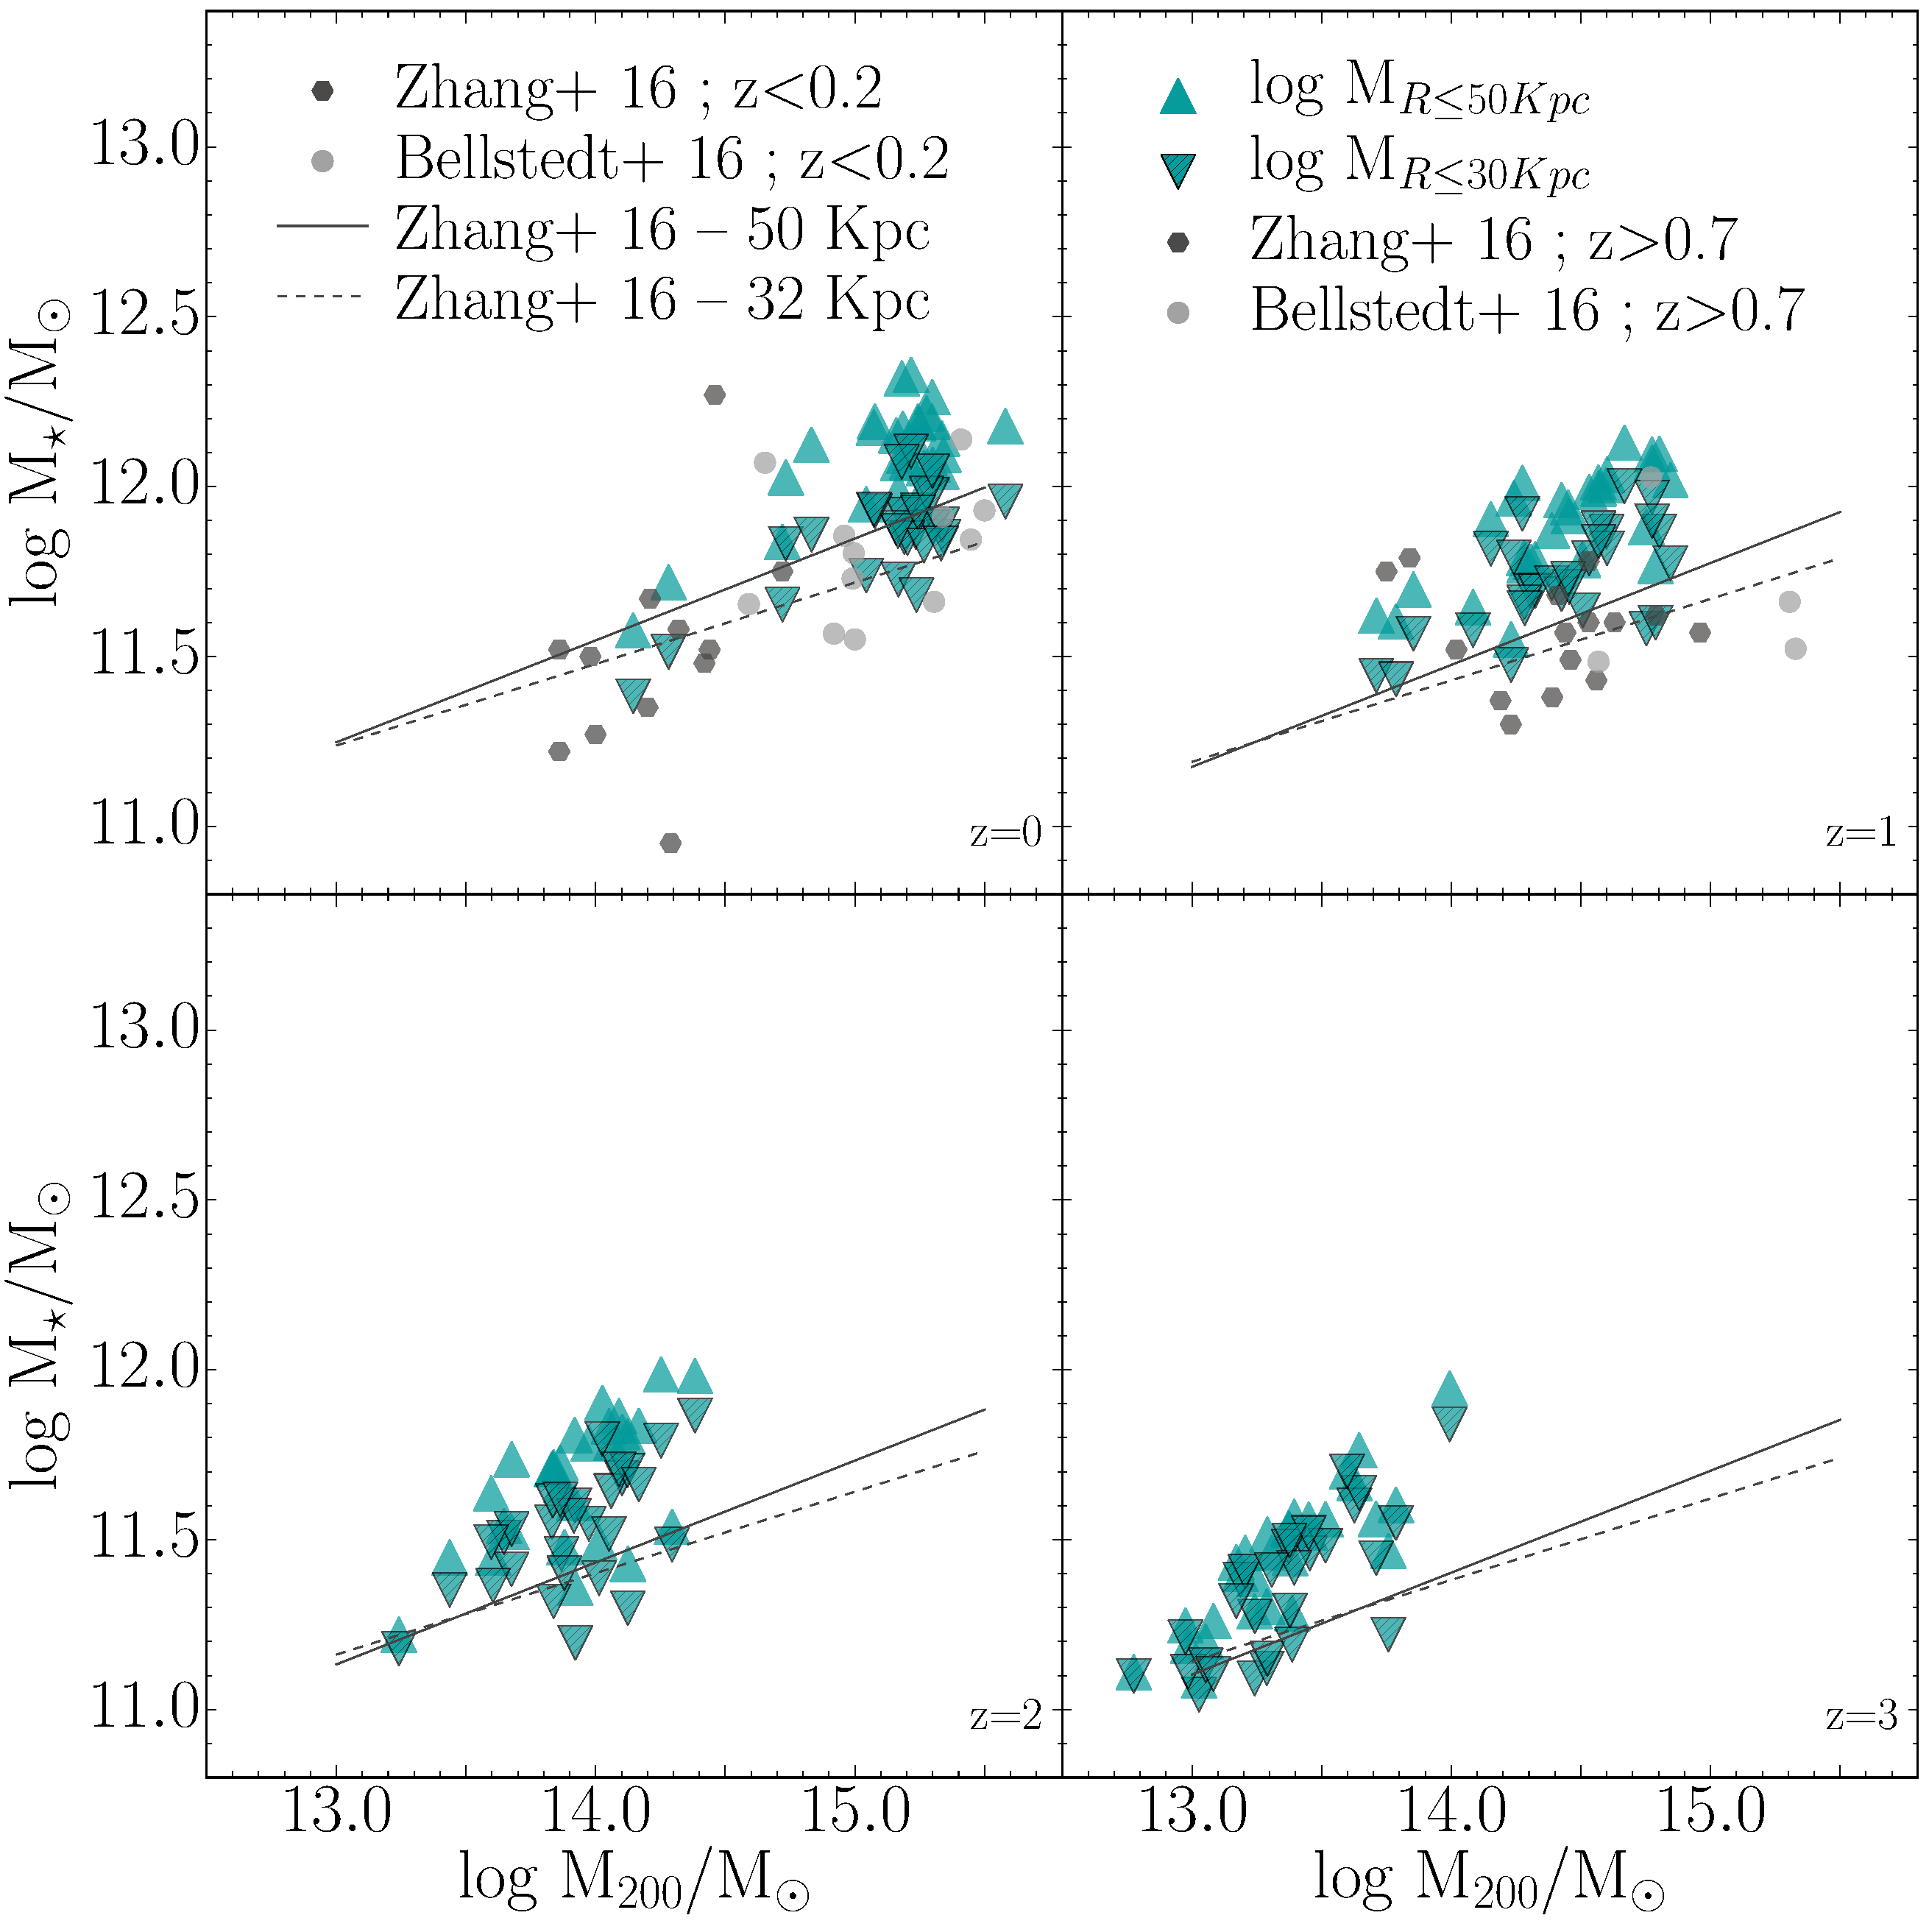
\includegraphics[height=12cm, width=13cm]{../al_final/LR/evolucion/relaciones/zhang_vs_z.pdf}
\end{figure}

ver: There is also a (weak) correlation between BCG mass and the mass of their host clusters, which does not change significantly
with redshift out to $z\sim 0.8 (Edge 1991; Collins & Mann 1998; Burke, Collins & Mann 2000; Brough et al. 2007; Stott et al. 2008;
Whiley et al. 2008).$

\section{evolucion en masa}

\begin{figure}[H]
 \centering
 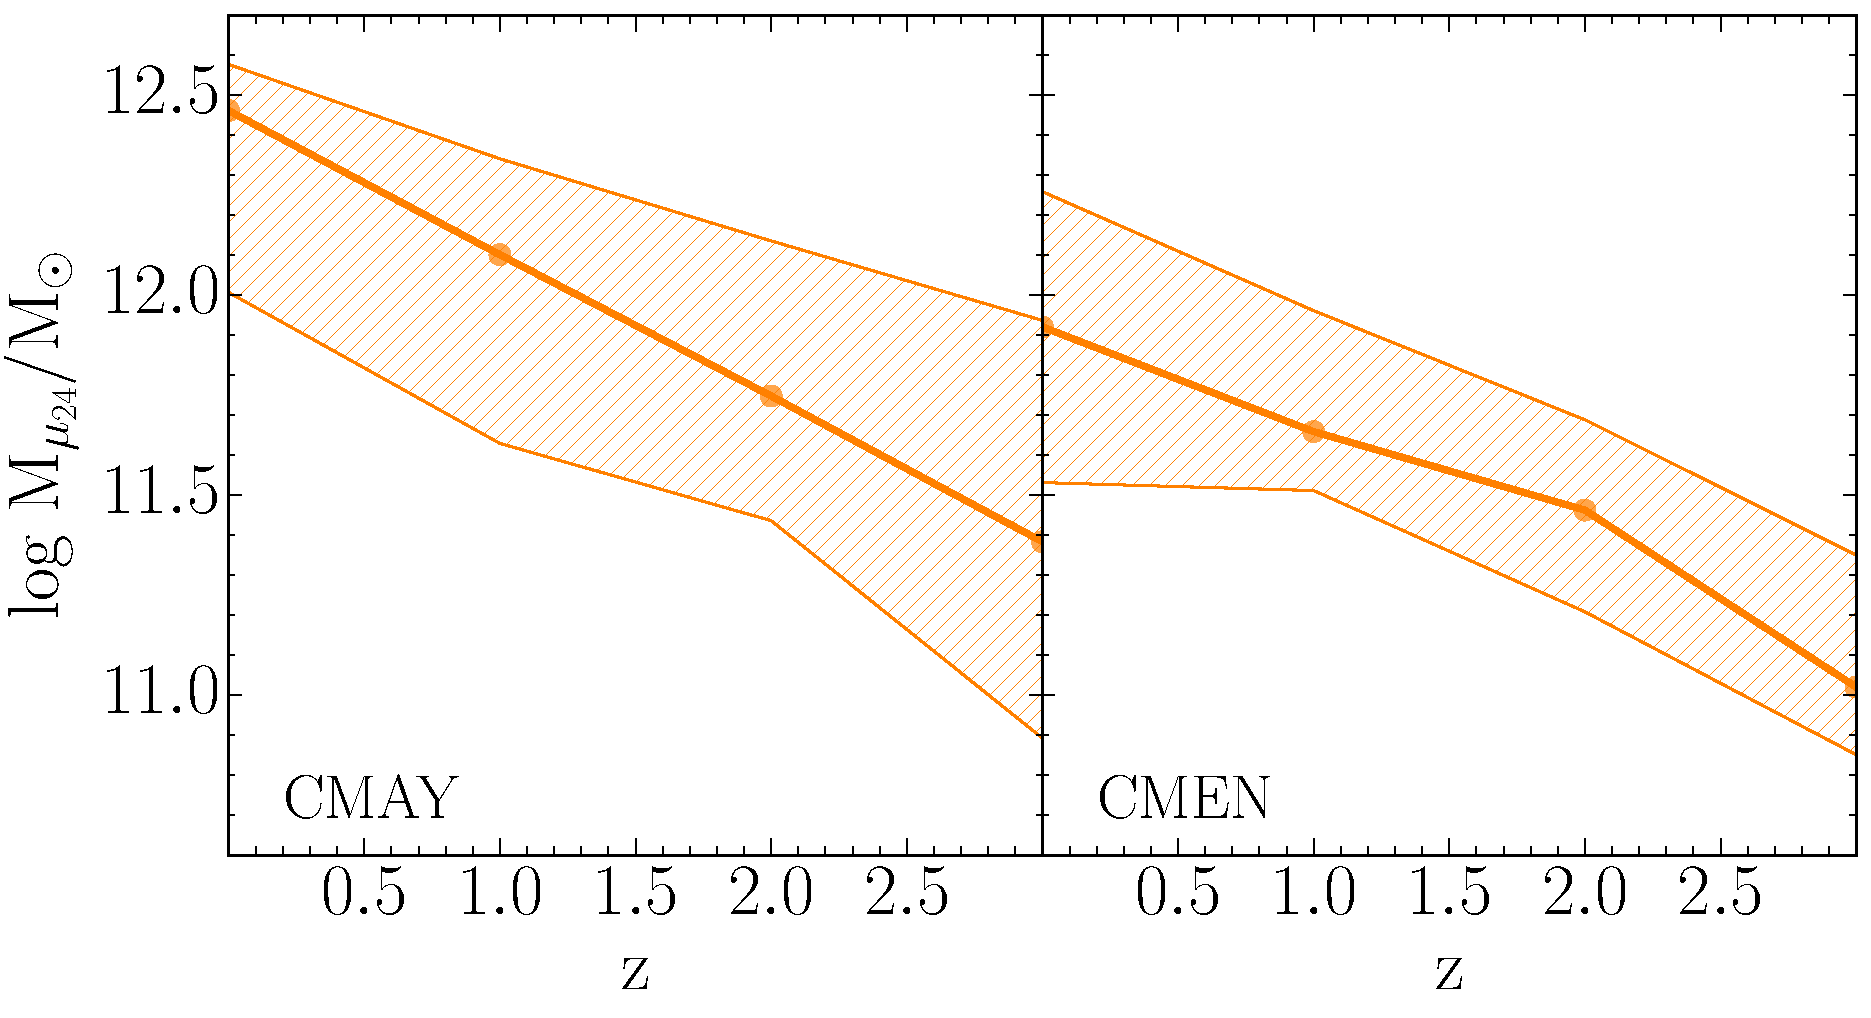
\includegraphics[height=7cm, width=14cm]{../al_final/LR/evolucion/observacional/evolucion_M24.pdf}
\end{figure}

\begin{figure}[H]
 \centering
 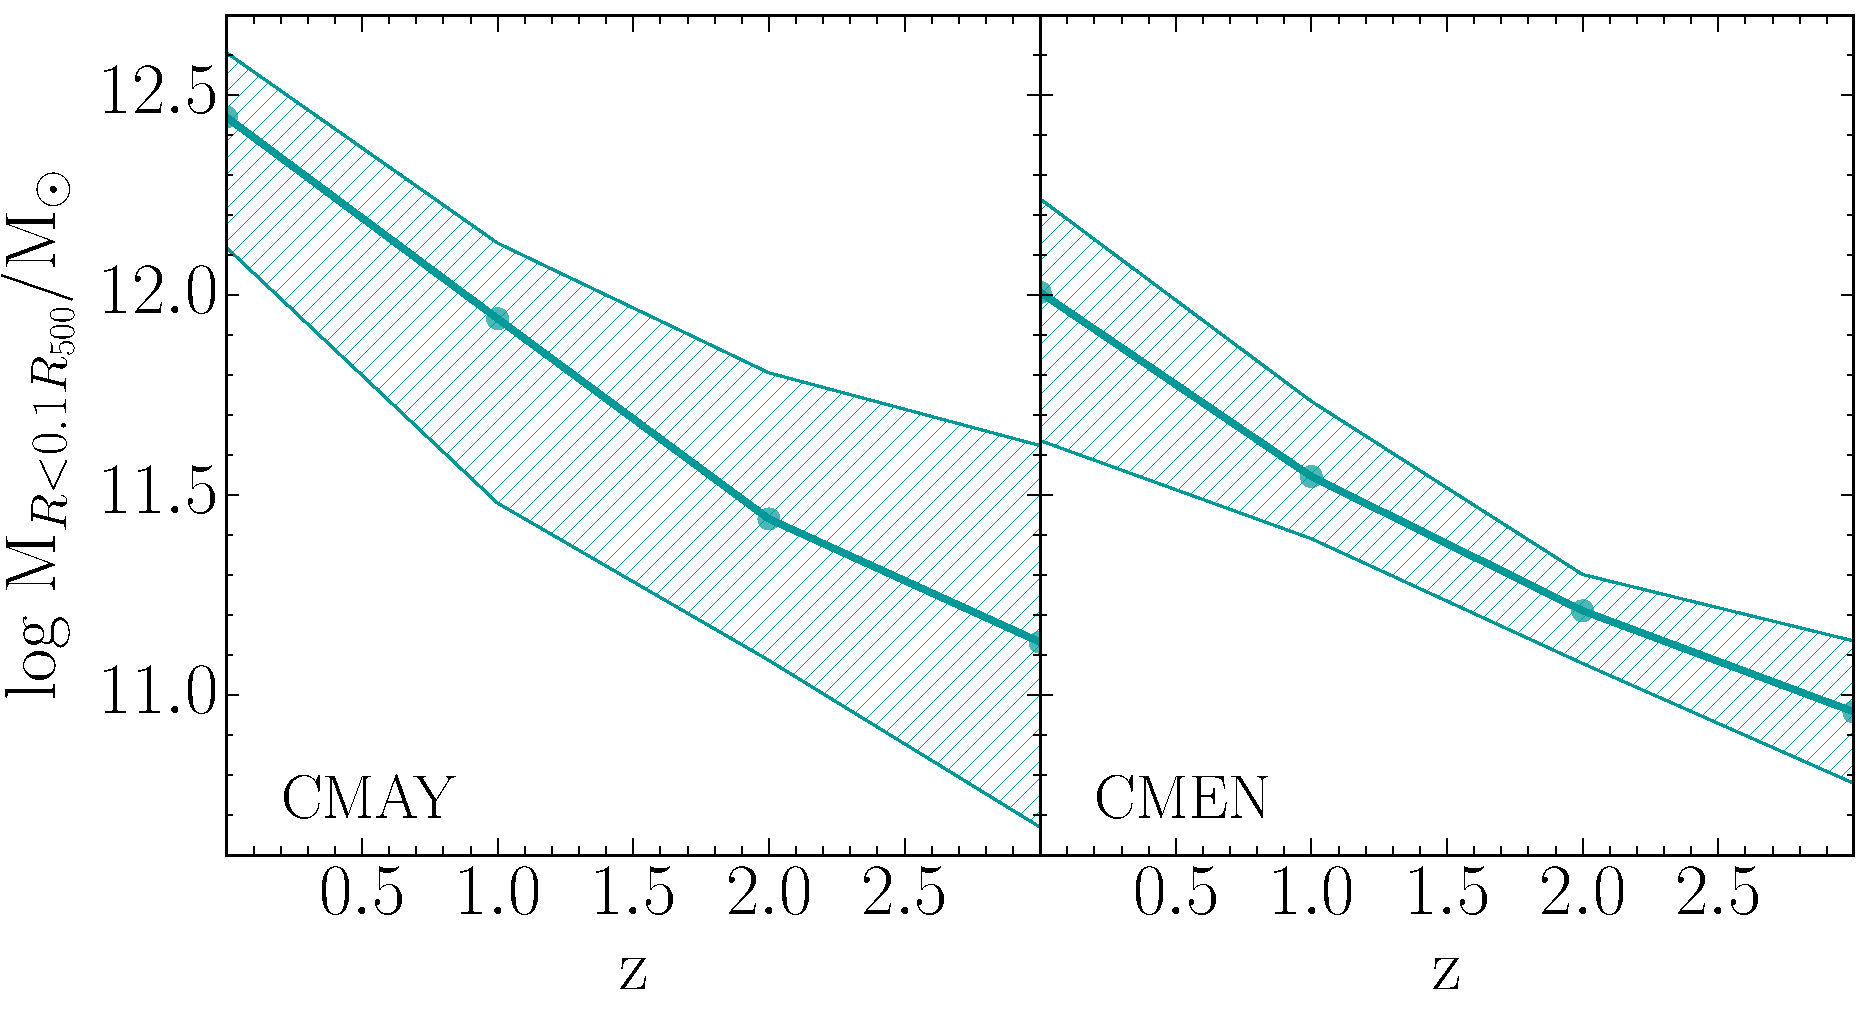
\includegraphics[height=7cm, width=14cm]{../al_final/LR/evolucion/simulacion/evolucion_M10_grandes_chicas.pdf}
\end{figure}


\begin{figure}[H]
 \centering
 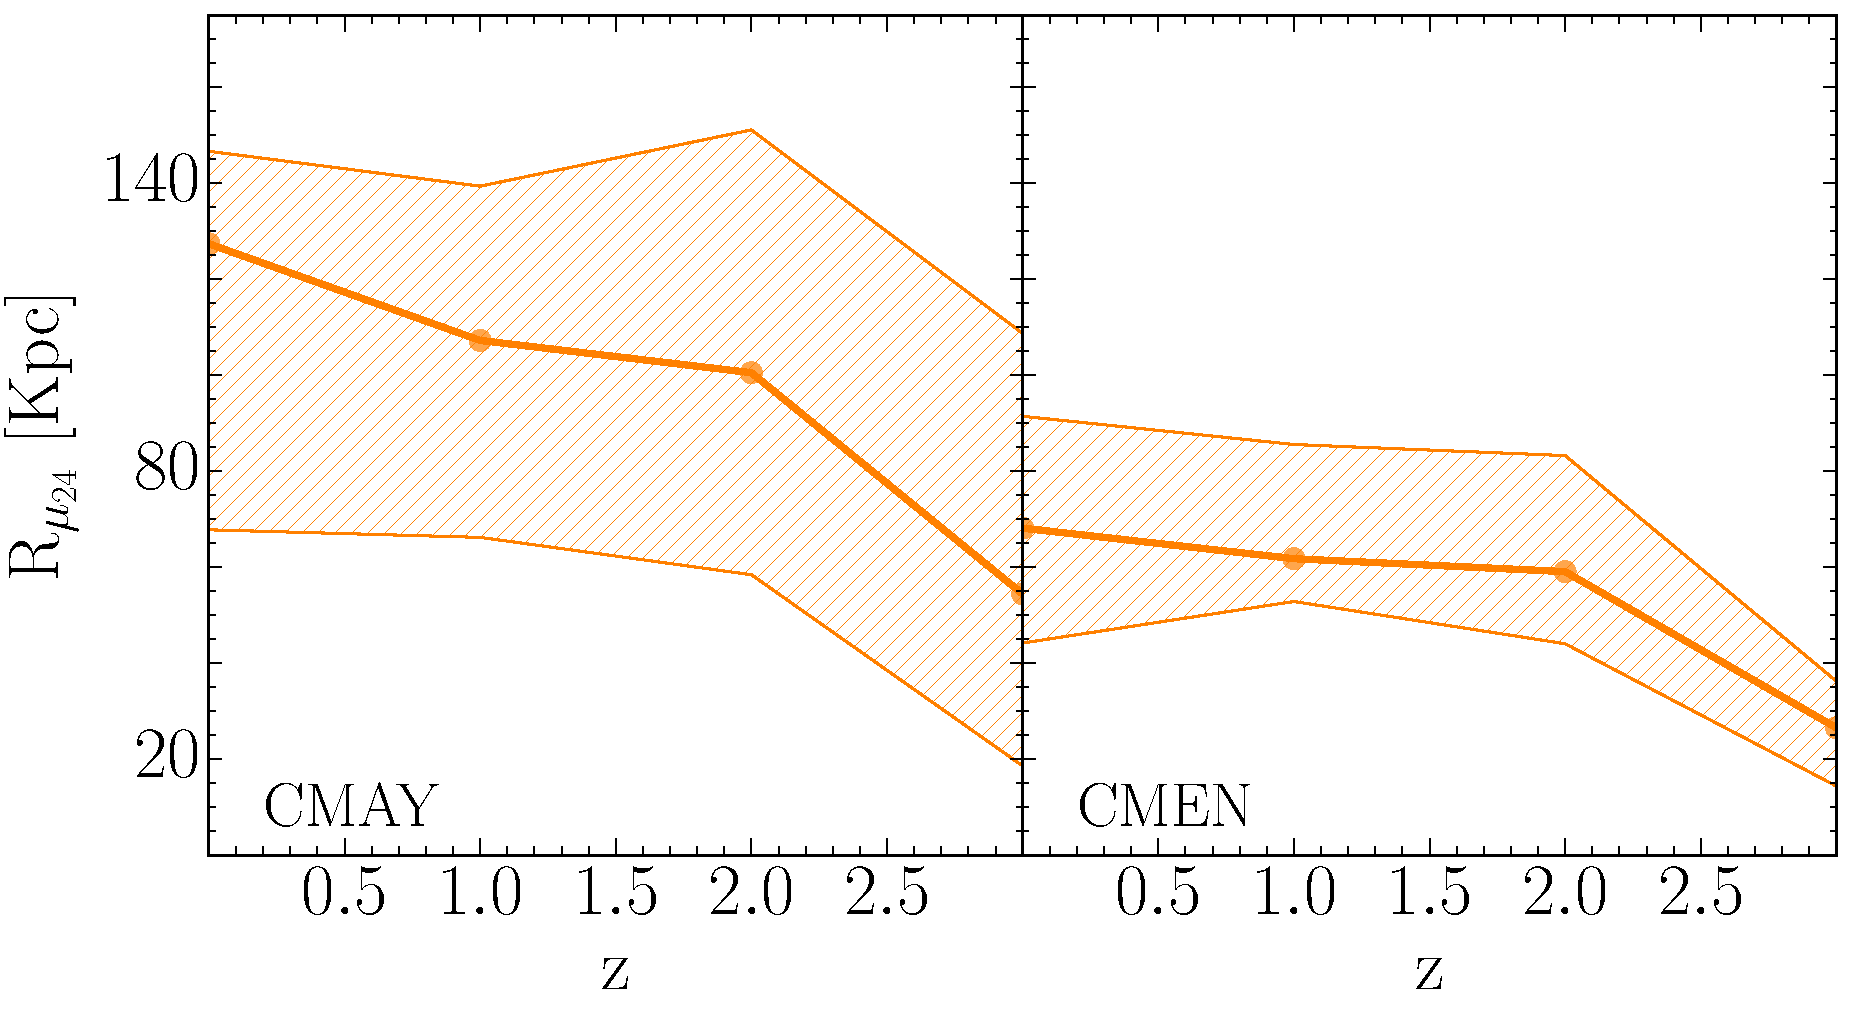
\includegraphics[height=7cm, width=14cm]{../al_final/LR/evolucion/observacional/evolucion_R24.pdf}
\end{figure}

\begin{figure}[H]
 \centering
 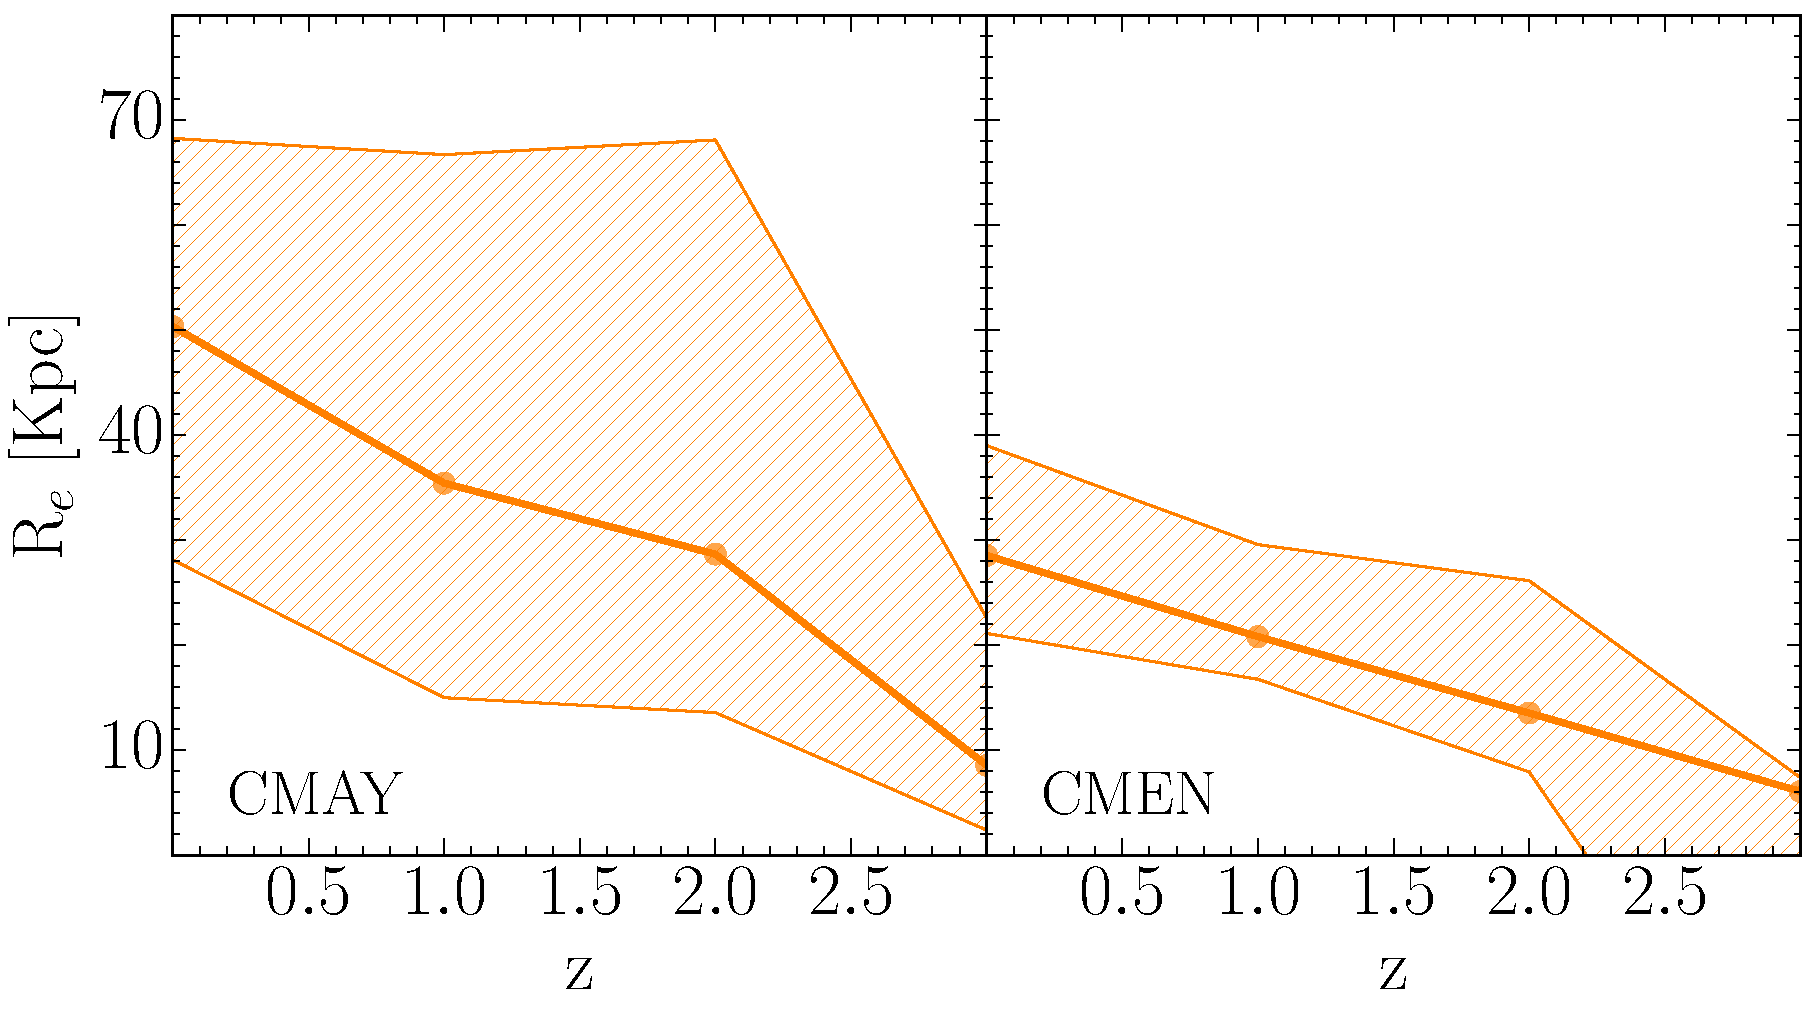
\includegraphics[height=7cm, width=14cm]{../al_final/LR/evolucion/observacional/evolucion_Re.pdf}
\end{figure}


\begin{figure}[H]
 \centering
 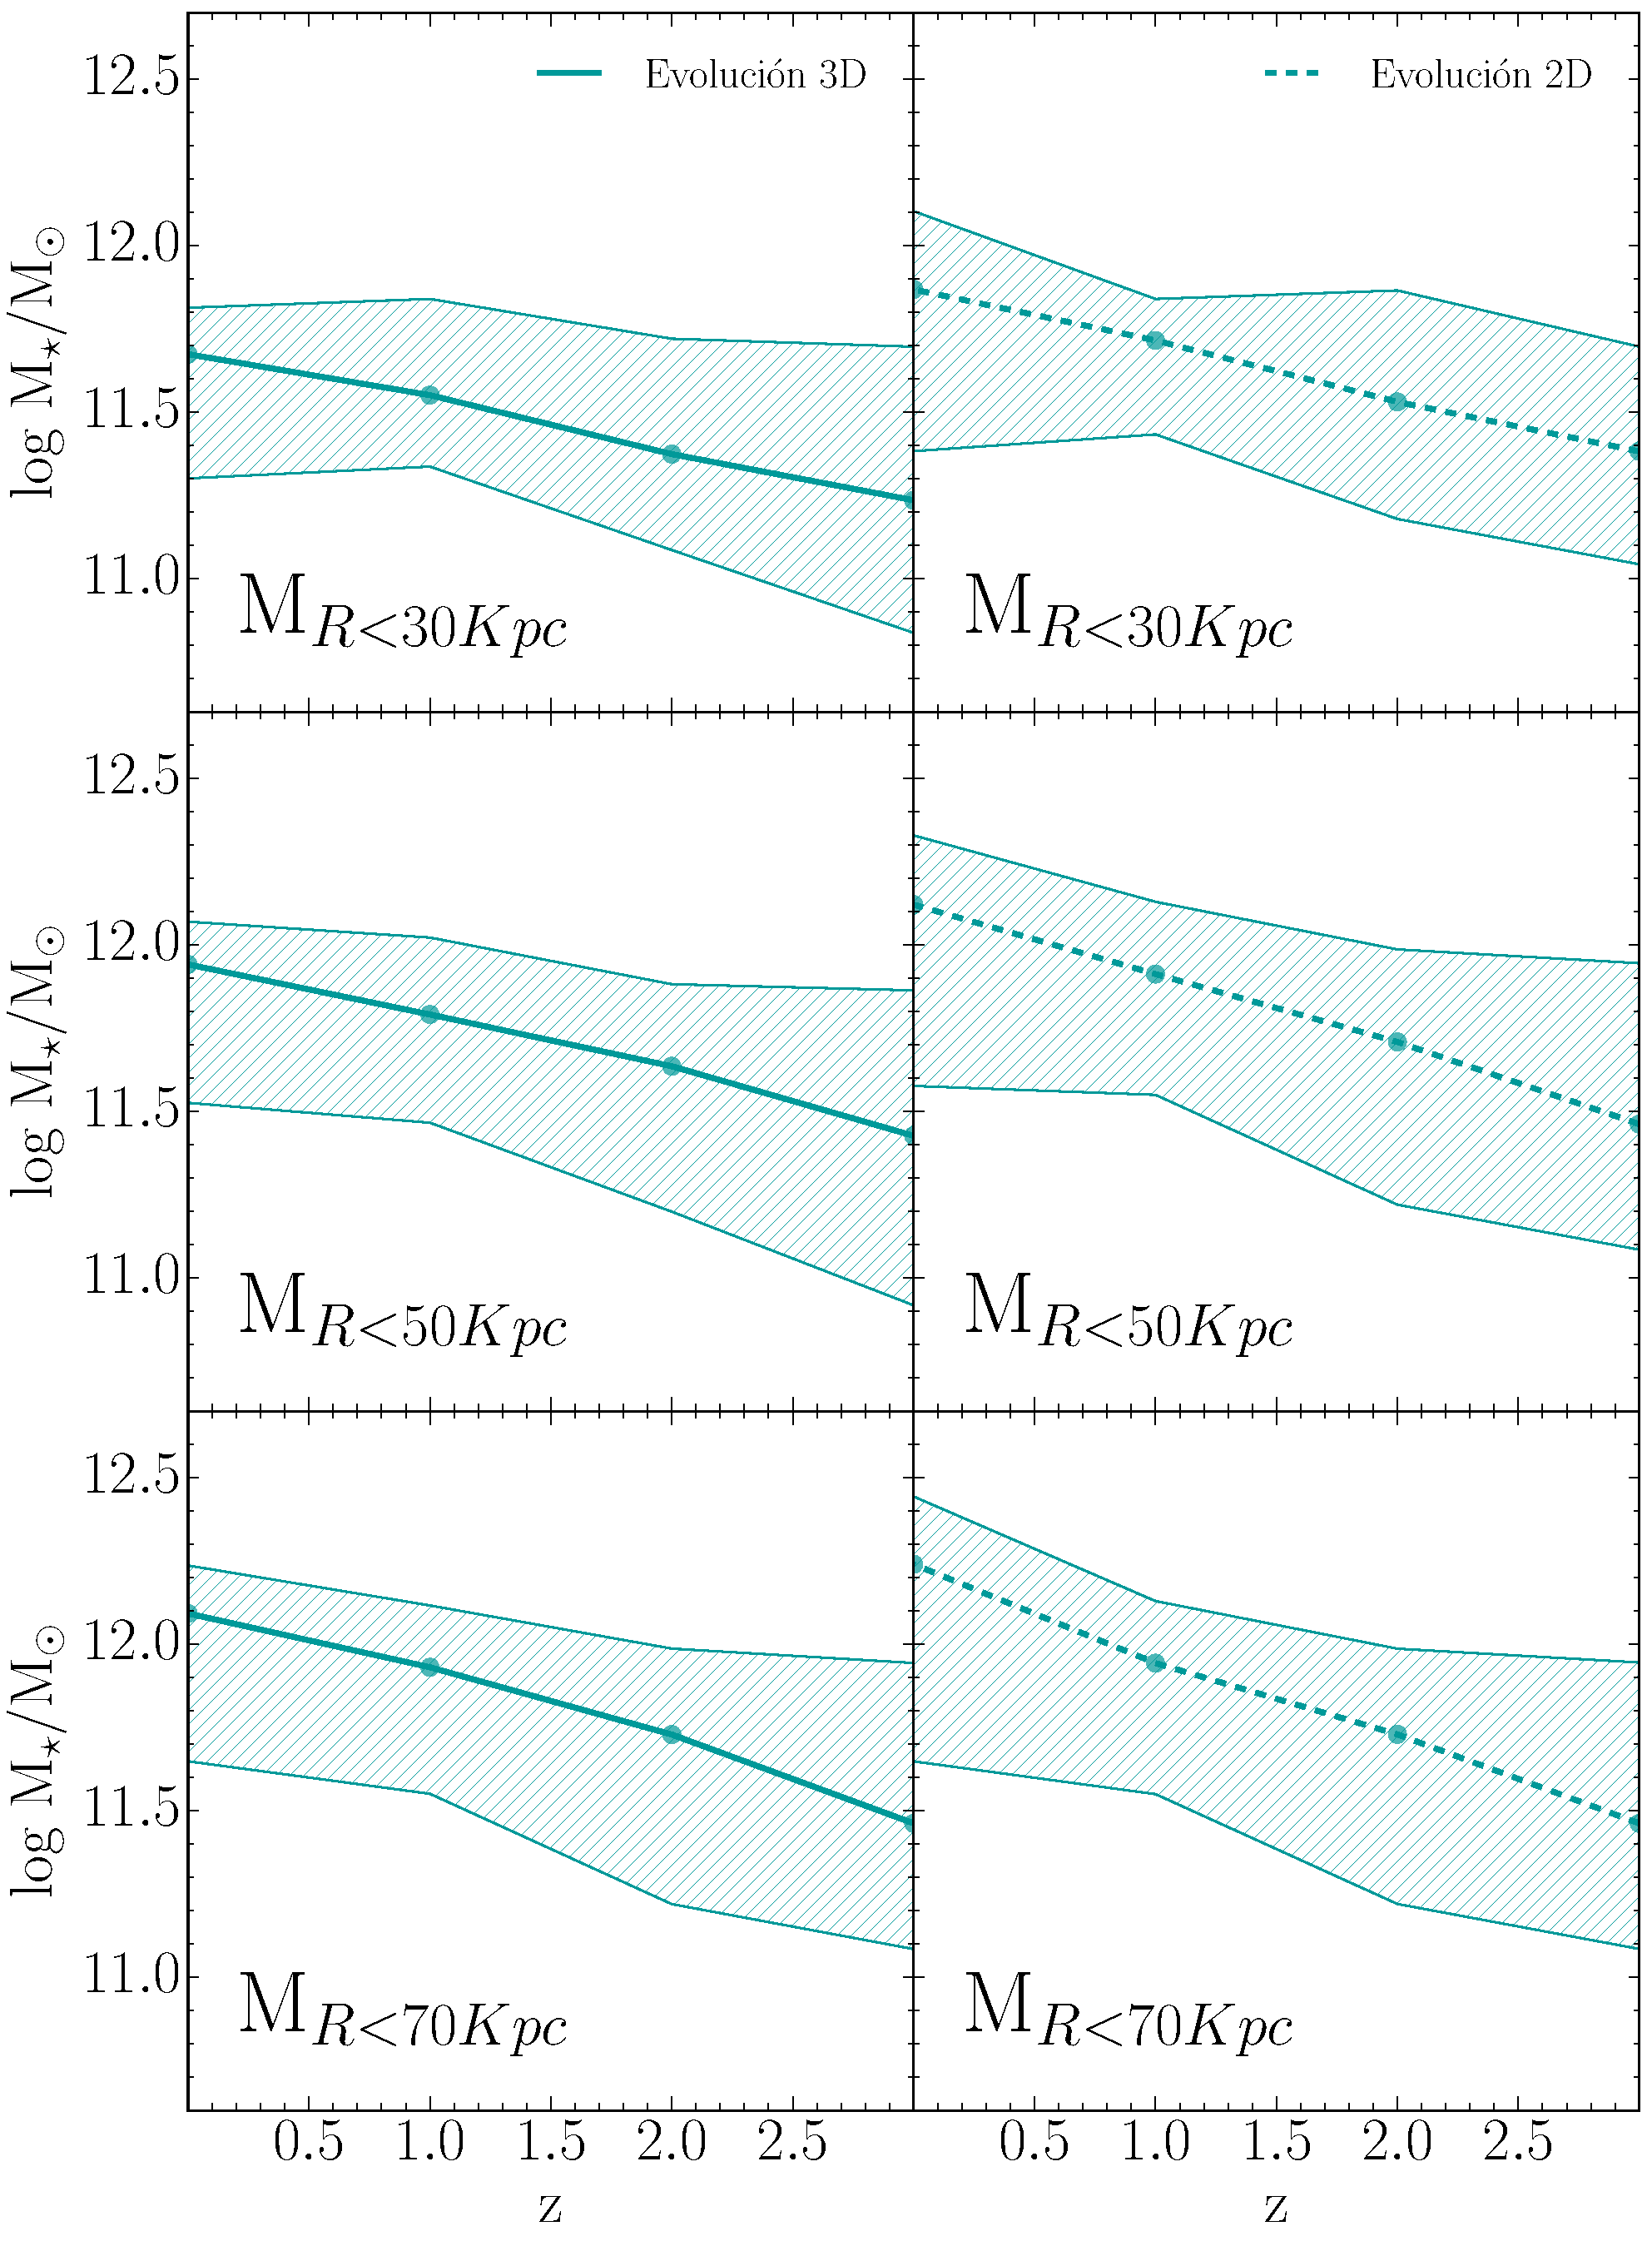
\includegraphics[height=18cm, width=14cm]{../al_final/LR/evolucion/simulacion/evolucion.pdf}
\end{figure}




\begin{figure}[H]
 \centering
 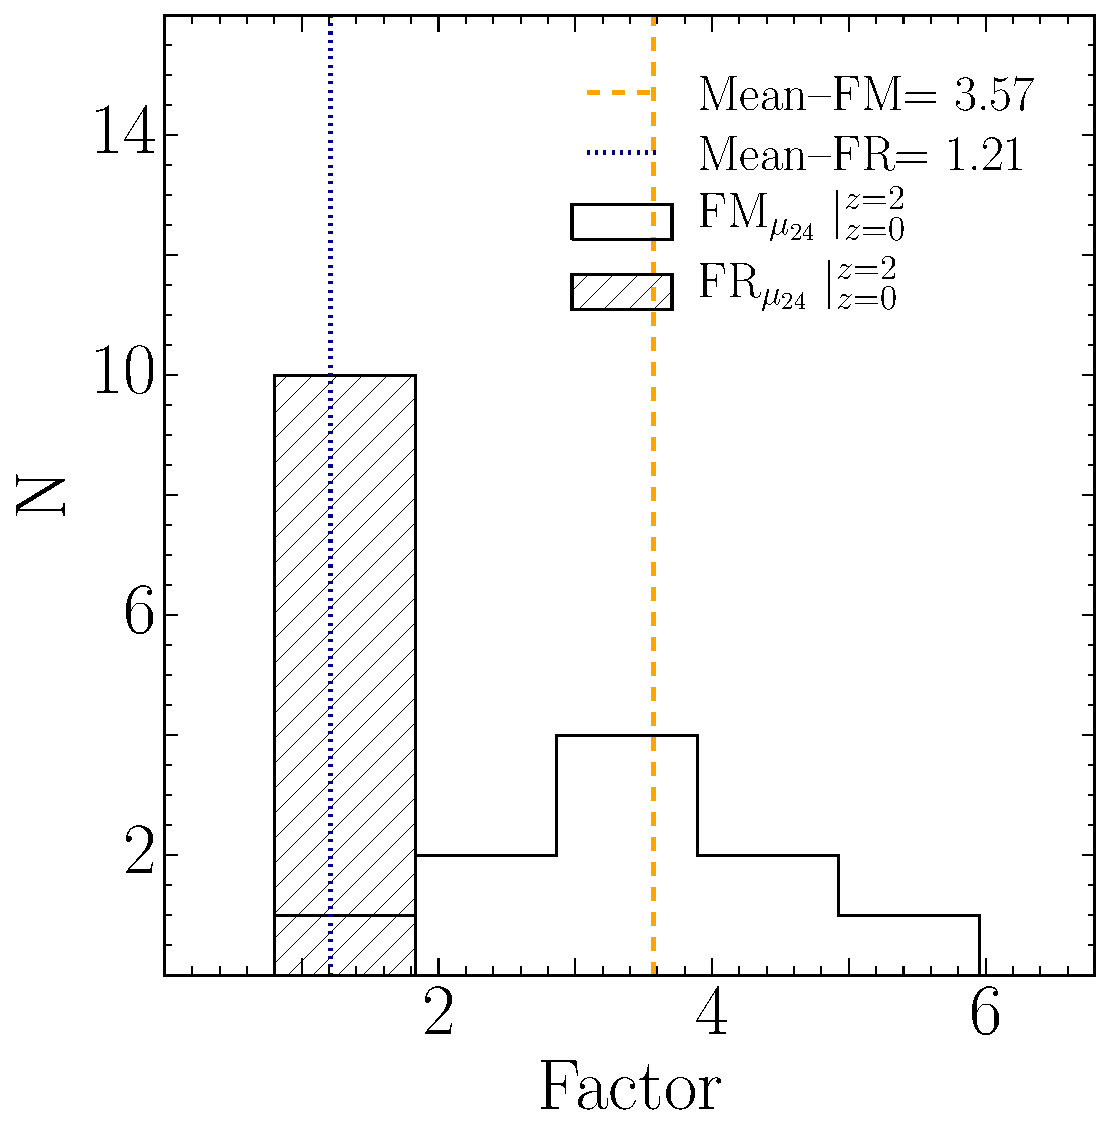
\includegraphics[height=7cm, width=7cm]{../al_final/LR/evolucion/histogramas/cocoientesmr24.pdf}
 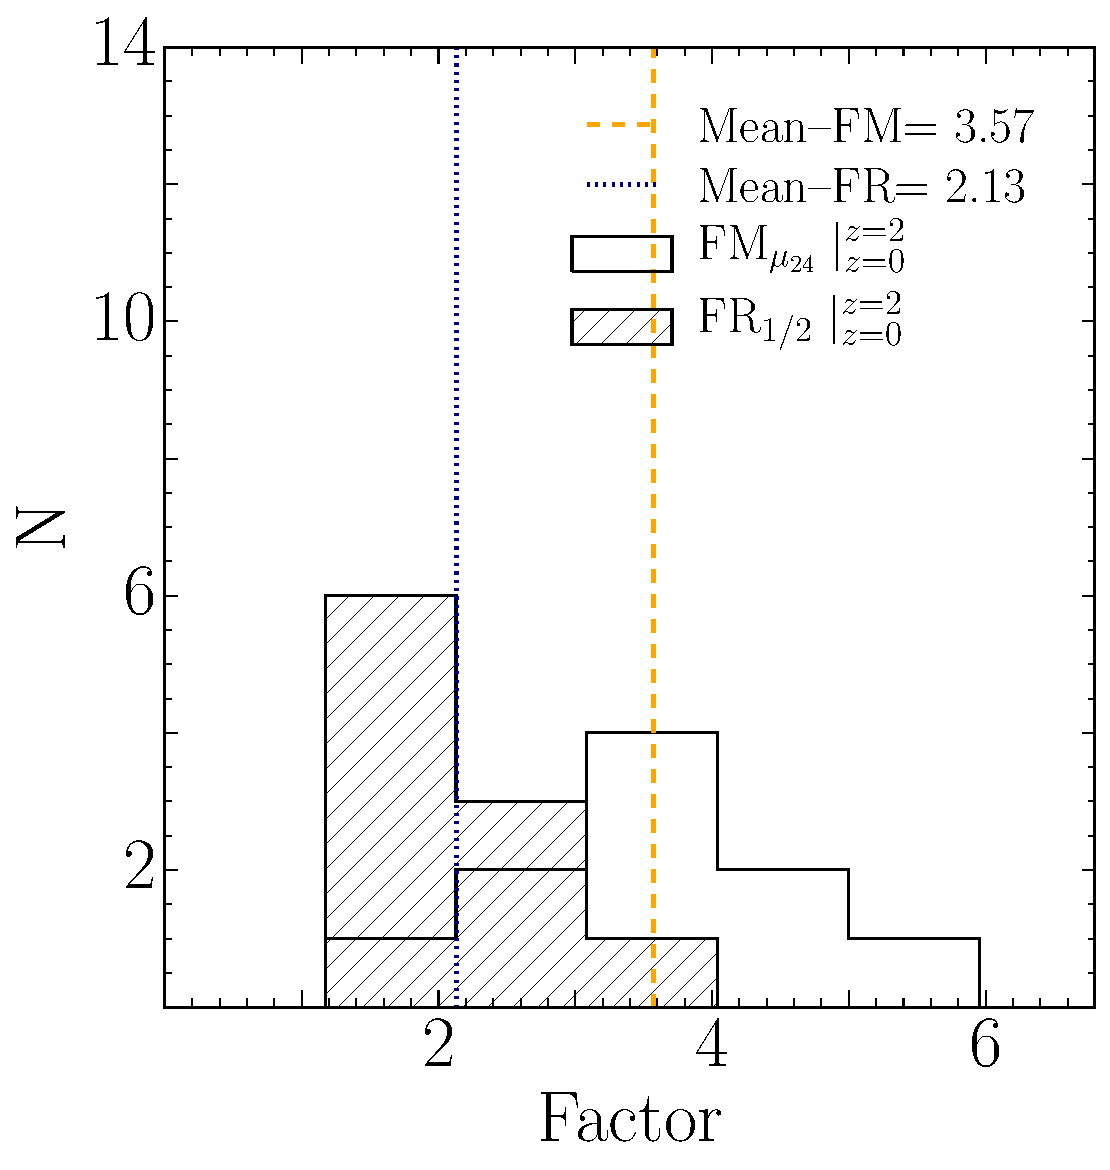
\includegraphics[height=7.2cm, width=7cm]{../al_final/LR/evolucion/histogramas/cocoientesmr1medio.pdf}
 \\
 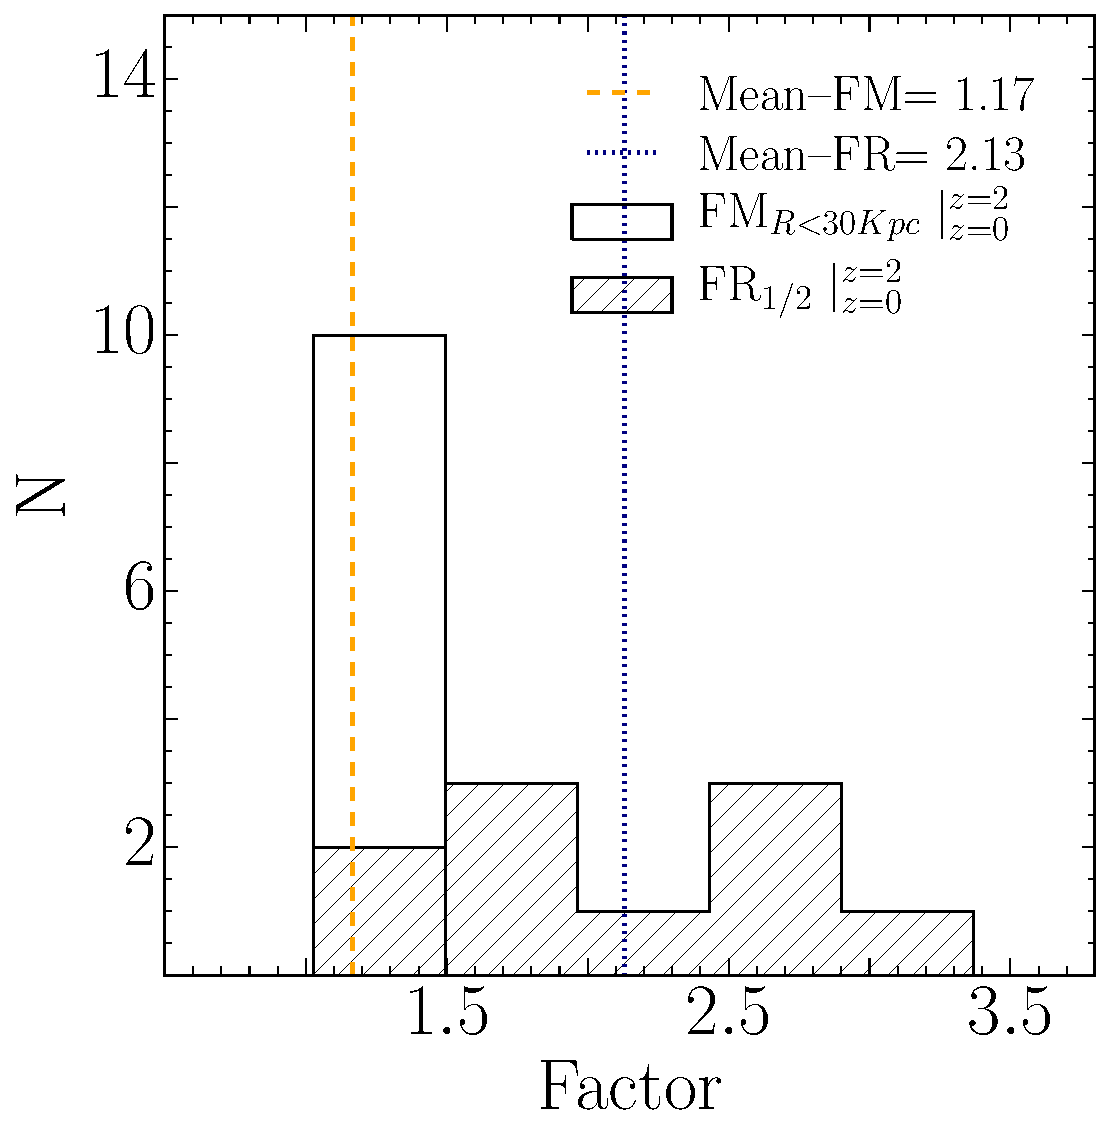
\includegraphics[height=7cm, width=7cm]{../al_final/LR/evolucion/histogramas/cocoientesm30r1medio}
 \includegraphics[height=7cm, width=7cm]{../al_final/LR/evolucion/histogramas/cocoientesm50r1medio}
\end{figure}


\section{evolucion en perfiles}

\begin{figure}[H]
 \includegraphics[height=24cm, width=15cm]{../al_final/plots/perfiles/bajustes_mues.pdf}
\end{figure}

\begin{figure}[H]
 \includegraphics[height=24.5cm, width=15cm]{../al_final/densidades/densidades.pdf}
\end{figure}



\section{edades y metalicidades}

\begin{figure}[H]
 \includegraphics[height=12cm, width=13cm]{../al_final/estrellas/stack/ultimoMETALICIDADES-PROG_zsunasplund.pdf}
\end{figure}

\begin{figure}[H]
 \includegraphics[height=12cm, width=13cm]{../al_final/estrellas/stack/ultimoEDADES-PROG_olivA.pdf}
\end{figure}


\begin{figure}[H]
 \includegraphics[height=7cm, width=7cm]{../al_final/estrellas/stack/ajustes/gradiente_edad_z0.pdf}
 \includegraphics[height=7cm, width=7cm]{../al_final/estrellas/stack/ajustes/gradiente_metalicidad_z0.pdf}
\end{figure}



\section{influencia del polvo. Solo a z=3 para algun dusty case}

\begin{figure}[H]
 \centering
 \includegraphics[height=7.5cm, width=7.5cm,trim={0cm   0.1cm 3.5cm 1.cm},clip ]{../al_final/LR/LR_minpot3_rmmax/nodust/grupo0/mu24/D1/026/maps_D1.pdf}
 \includegraphics[height=7.5cm, width=7.5cm,trim={2.8cm 0.1cm 0.3cm 1.cm},clip ]{../al_final/LR/LR_minpot3_rmmax/dust/grupo0/mu24/D1/026/maps_D1.pdf}
\end{figure}


\begin{figure}[H]
 \centering
 \includegraphics[height=7.5cm, width=7.5cm,trim={0cm   0.1cm 3.5cm 1.cm},clip ]{../al_final/LR/LR_minpot3_rmmax/nodust/grupo0/mu24/D22/026/maps_D22.pdf}
 \includegraphics[height=7.5cm, width=7.5cm,trim={2.8cm 0.1cm 0.3cm 1.cm},clip ]{../al_final/LR/LR_minpot3_rmmax/dust/grupo0/mu24/D22/026/maps_D22.pdf}
\end{figure}

\begin{figure}[H]
 \includegraphics[height=8.5cm, width=8.5cm,trim={0cm 0.1cm 0.cm 0.cm},clip]{../al_final/LR/LR_minpot3_rmmax/polvo_nopolvo1b3.pdf}
 \includegraphics[height=8.5cm, width=7.1cm,trim={2.9cm 0.1cm 0.2cm 0.cm},clip]{../al_final/LR/LR_minpot3_rmmax/polvo_nopolvo1D22.pdf}
\end{figure}


\begin{figure}[H]
\centering
 \includegraphics[height=8.5cm, width=8.5cm,trim={0cm 0.1cm 0.cm 0.cm},clip]{../al_final/plots/seds/plots_seds/sed_D1.pdf}
 %\includegraphics[height=8.5cm, width=7.1cm,trim={2.9cm 0.1cm 0.3cm 0.cm},clip]{../al_final/plots/seds/plots_seds/sed_D22.pdf}
\end{figure}


\begin{figure}[H]
 \centering
 \includegraphics[height=9cm, width=9cm]{../al_final/LR/evolucion/histogramas/Mmu_polvo_vs_nopolvo.pdf}
\end{figure}


\section{Estabilidad a High Resolution}
\begin{figure}[H]
 \centering
 \includegraphics[height=10cm, width=11cm]{../al_final/LR/evolucion/MRvsLR/mr_vs_lr.pdf}
\end{figure}

\begin{figure}[H]
 \hspace*{-1.4cm}\includegraphics[height=6.cm, width=6.3cm    ,trim={0cm   0.1cm 4.7cm 1.38cm},clip ]{../al_final/LR/LR_minpot3_rmmax/nodust/grupo0/mu24/D2/091/contoursmaps125.pdf}
  \hspace*{-.1cm}\includegraphics[height=6.cm, width=5.2cm,trim={2.5cm 0.1cm 4.7cm 1.38cm},clip ]{../al_final/MR/MR_minpot3_rmmax/nodust/grupo0/mu24/D2/091/contoursmaps125.pdf}
  \hspace*{-.1cm}\includegraphics[height=6.cm, width=6.9cm,trim={2.5cm 0.1cm 0.3cm 1.38cm},clip ]{../al_final/HR/HR_minpot3_rmmax/nodust/grupo0/mu24/D2/091/contoursmaps125.pdf}
\end{figure}


\begin{figure}[H]
  \hspace*{-1.4cm}\includegraphics[height=6cm, width=6cm,trim={0cm   0.cm 0.cm 0.cm},clip ]{../al_final/resoluciones/res1.pdf}
  \hspace*{.1cm}\includegraphics[height=6cm, width=5.4cm ,trim={2.3cm  0.cm 0.cm 0.cm},clip ]{../al_final/resoluciones/res2.pdf}
  \hspace*{.1cm}\includegraphics[height=6cm, width=5.4cm ,trim={2.3cm  0.cm 0.cm 0.cm},clip ]{../al_final/resoluciones/res3.pdf}
\end{figure}

\section{Relaciones de Escala}



\begin{figure}[H]
 \centering
 \includegraphics[height=9.5cm, width=10cm]{../al_final/plots/parametros_de_escala/mevsm_medians.pdf}
\end{figure}

\begin{figure}[H]
 \centering
 \includegraphics[height=9.5cm, width=10cm]{../al_final/plots/parametros_de_escala/nvsm_medians.pdf}
\end{figure}

\begin{figure}[H]
 \centering
 \includegraphics[height=9.5cm, width=10cm]{../al_final/plots/parametros_de_escala/revsm_medians.pdf}
\end{figure}

\begin{figure}[H]
 \centering
 \includegraphics[height=10cm, width=11cm]{../al_final/plots/parametros_de_escala/kormendy.pdf}
\end{figure}
